\def\ReadCommandLineArg#1 {%
  \def\CommandLineArg{#1}%
  \input{\jobname}}
\unless\ifdefined\CommandLineArg
\endinput\expandafter\expandafter\expandafter\ReadCommandLineArg\fi

\documentclass[12pt]{article}

\usepackage[utf8]{inputenc}
\usepackage{amsfonts}
\usepackage{amsmath}
\usepackage{graphicx}
\usepackage{textgreek}
\usepackage{fancyvrb}
\usepackage[toc,page]{appendix}
\usepackage{subfigure}
\usepackage{geometry}
\usepackage{longtable}
\usepackage{float}
\usepackage{booktabs}
\usepackage{hyperref}
\usepackage{tikz}
\usepackage{xcolor}
\usepackage{caption}

\setlength\LTleft{0in}
\setlength\LTright{0in}
% \setcounter{LTchunksize}{10}

\makeatletter
\def\IfClass#1#2#3{\@ifundefined{opt@#1.cls}{#3}{#2}}
\newif \ifIEEEtran \@ifclassloaded{IEEEtran} {\IEEEtrantrue} {\IEEEtranfalse}
\makeatother

\DefineVerbatimEnvironment{juliaout}{Verbatim}{}
\DefineVerbatimEnvironment{juliacode}{Verbatim}{fontshape=sl}
\DefineVerbatimEnvironment{juliaterm}{Verbatim}{}

\title{\Large \bf Inexact MDL for Linear Manifold Clusters}
\author{Robert M. Haralick, Art Diky, Xing Su, Nancy Y. Kiang}

\begin{document}
\maketitle
\begin{abstract}

We present a regularization technique based on the minimum description length
(MDL) principle for the linear manifold clustering. We suggest an inexact minimum
description length method based on describing the data structure as
linear manifold clusters.
We examine the behavior of the proposed method and compare it performance
against simulated clustering results of various dimensionality and structure.
Finally, we empirically evaluate the proposed technique on a climate data.

\end{abstract}
     % Abstract
\tableofcontents
% -*- root: inexact_mdl_lmc.tex -*-
\section{Introduction}\label{sc:intro}

Minimum Description Length (MDL) can be understood to be a technical specification
or formalization of the Occam's razor principle to understand a data set.
One way to pose the general problem is given a data set, define a language in
which to represent the data set so that the data set described in the language
is a meaningful description and the number of bits for the representation in
the language is minimal. This is different from data compression in the sense
that data compression only uses information theoretic methods to minimize the
number of bits to represent the data set, but the representation in itself
is not meaningful. It does not give any insight into the structure of the data.
\IfClass{IEEEtran}{}{
By first defining a language which is capable of representing the data and
the structure of the data in a meaningful way, minimum description length does
compress the data and simultaneously provides the structure of the data as well.
}
If there are multiple possible languages for describing the data, minimum
description length can be the principle for deciding which is the best language.

\IfClass{IEEEtran}{}{
It is easy to give an example of data that has a structure. Consider a data set
upon which it is appropriate to do linear regression. So there are $K$ observations
of the values of $N$ independent variables in which the values are considered
to have no error. For each of the $K$ observations, there is one dependent
variable whose value is considered to be noisy. The linear regression context
assumes that the dependent variable is a linear combination of the $N$ independent
variables. This linear combination is the structure of the data. However,
regression only provides the estimates of the linear combination and the total
squared error. So we have the structure of the data but we do not know the values
of the $K$ observations of the dependent variable. An MDL approach would define
the language to be the language of linear combinations. It would assume that
the $K$ observations of the $N$ independent variables are known precisely and
do not enter into the MDL description. It would then represent the $K$ observations
of the dependent variable. But instead of representing these $K$ observations
independent of the linear combination data structure, it would represent each
value of the dependent variable in terms of the difference between its actual
value and the value that would be estimated using the data structure.
These differences would then be encoded in an efficient information theoretic
way based on entropy.
}


% In this paper we develop an inexact minimum description length method for
% describing the structure of the data in terms of linear manifold clusters.
Our description language is the language of linear manifolds. Each linear
manifold cluster consists of the description of the linear manifold and
the coding of the data associated with the linear manifold is given by encoding
the orthogonal projection of each data point onto its manifold and the encoding
of the difference between its position off the manifold and its orthogonal
projection on the manifold. The inexactness of the description arises because
the description of the position of each data point off the manifold is
described not exactly, but with some controlled error.


Section \ref{sc:lit-review} is a literature review. Section \ref{sc:lmclus}
is a technical description of the linear manifold clustering stochastic search
technique. Section \ref{sc:mdl-lmclus} describes how the MDL principle is used
to determine whether to accept a cluster or not. Section \ref{sc:results}
discusses our results and section \ref{sc:conclusion} concludes the paper.
        % Introduction
% -*- root: inexact_mdl_lmc.tex -*-
\section{Literature Review}
\label{sc:lit-review}
\IfClass{IEEEtran}
{
Subspace clustering \cite{Kriegel:2009fj} is a special case of linear manifold
clustering, where the basis vector set for each cluster is a subset of
the natural basis vectors of the space.
%
Data can be well approximated by a mixture of linear manifolds (linear or affine
subspaces).
}{
The main challenge for clustering in high-dimensional spaces is that different
subsets of points are relevant for different clusters, but cluster points,
originally in the full space, associated with various subspaces. Moreover,
various correlations between points are relevant to different clusters.
Variety of subspace and correlation clustering algorithms try to find clusters
in axis-aligned and arbitrarily oriented subspaces \cite{Kriegel:2009fj}.
%
Because, there are infinite number of subspaces, additional assumptions are
required to overcome infinite search space. One of the assumptions is that
high-dimensional observations lie on or close to multiple smooth low-dimensional
manifolds embedded in a full space of dataset. Thus, viewing cluster as
a collection of points on or near a compact manifold becomes a reasonable and
promising extension of traditional centroid-based clustering methods, which
leads to manifold clustering.
%
Data can be well approximated by a mixture of linear manifolds (linear or affine
subspaces).  Such assumption leads to a large number of linear manifold
clustering methods.
}
Haralick and Harpaz \cite{Haralick:2007rt} presented a linear manifold
clustering algorithm (LMCLUS), which is a strict partitioning clustering
algorithm, that performs stochastic search on the dataset in order to find best
possible location of the linear manifold clusters.
Kak \cite{Kak:2016KP} used a linear manifold representation of a fixed number of
clusters, obtained by sampling the original dataset and minimizing
the reconstruction error from point assignments to cluster prototypes.
Peng et al. \cite{Peng:2013PZ} constructed linear manifold cluster prototypes by
performing spectral decomposition of small random samples with subsequent
assignment of the rest of the dataset points to a nearest subspace cluster
prototype. Wang et al. \cite{Wang:2011yu} used a mixture of probabilistic PCAs
to form a collection of linear manifolds on the dataset.
\IfClass{IEEEtran}{}{
These linear manifolds were
used to reconstruct non-linear manifolds, that reflect local geometric
information of the data, and from a suitable affinity matrix that served as
input for spectral clustering technique.}

Moreover, many linear methods fail to provide good performance when applied to
nonlinear structures. On the other hand, nonlinear methods, such as nonlinear
dimensionality reduction techniques, can be naturally used on linear manifolds
\IfClass{IEEEtran}{\cite{Souvenir:2005pr, Goh:2008vr,Subbarao:2006SM}.}{.}
\IfClass{IEEEtran}{}{
Souvenir \cite{Souvenir:2005pr} used non-linear dimensionality reduction, i.e.
multidimensional scaling, to construct low-dimensional embedding, a non-linear
manifold, of the original data that was consequently partitioned by EM
clustering algorithm.
Goh and Vidal \cite{Goh:2008vr} used a Locally Linear Embedding (LLE) reduction
technique, that used the Riemannian distance, of the original data to construct
smooth low-dimensional manifolds representation for consequent spectral
clustering.
Subbarao and Meer \cite{Subbarao:2006SM} took more general approach in
describing manifold structures on data. They used a particular type of analytic
manifolds, Grassmann manifolds, to approximate geodesic distance on the manifold
structure which was used in conjunction with the mean shift clustering algorithm.
%
One of challenges when working with manifold clustering techniques is
an uncertainty related to the selection of the dimensionality of the manifold
embedding. As many algorithms, LMCLUS  does not know the dimensions of
the embedded manifold clusters before seeing the data. The original solution
in \cite{Haralick:2007rt} was to look through all subspace dimensions starting
from lowest. However, such an approach creates a problem - a dominance of
a high-dimensional clusters.
%
There is high probability that a high-dimensional subspace is selected over
a low-dimensional subspace when a cluster is constructed. This happens because
the relative distance between the farthest point and the nearest point converges
to 0 with increasing dimensionality \cite{Aggarwal:2001hk}, which results in
very tight separation bounds for high-dimensional candidate clusters that allows
them to pass a cluster formation criteria more often then for a low-dimensional
candidate.
%
Our solution  addresses the problem of the selection of
a high-dimensional manifold preference by introducing a regularization technique
based on a minimum description length (MDL) value of the prospective cluster.
The minimum description length principle is a method for inductive
inference that provides a generic solution to the model selection problem.
MDL is based on the following insight: any regularity in the data can be used
to compress the data, that is, to describe it using fewer symbols than
the number of symbols needed to describe the data literally \cite{Hansen:2001HY}.
The minimum description length (MDL) principle can be used in clustering to
discover underlying regularities, that are common to all the members of a group,
and an internal validation of the cluster goodness \cite{Kontkanen:2005pm, Georgieva:2011tk}.
}

Rissanen at al. \cite{Rissanen:2005RT} presented an approach where data and
noise are separated, and the code length of the model is restricted by a
parameter. The hypothesis selected by MDL captures all the structure inherent in
the data. Given the hypothesis, the data cannot be distinguished from random
noise.
\IfClass{IEEEtran}{}{
Therefore, it may be taken as a basis for lossy data compression: rather
than sending the whole sequence, we only send the hypothesis representing the
``structure'' in the data. The receiver can then use this hypothesis to generate
``typical'' data for it - this data should look statistically just the same as
the original data.
}
   % Literature Review
\section{Linear Manifold Clustering}
\label{sc:lmclus}

The cluster ideal in Linear Manifold Clustering is a linear manifold.
A linear manifold of dimension zero is a point. A linear manifold of dimension 1
is a line. A linear manifold of dimension 2 is a plane. In general,
a linear manifold is a translated subspace.
The dimension of the linear manifold is the dimension of the subspace.
K-means is a special case of linear manifold clustering where
the linear manifold has dimension zero.

Linear manifold clustering is appropriate in the case that there are
linear dependencies among the variables, each cluster having a different number
and different kinds of linear dependencies.
Let us take an example to make this clear.  Suppose that we are in a three
dimensional space with three clusters. The first two clusters have one linear
dependency. Their  linear manifolds  are planes.
In our example the planes are parallel. The third cluster has
two linear dependencies. Its linear manifold is a line. The observed data points
can be thought of as points whose ideals are on their manifolds, but were
slightly perturbed off their manifolds, see Fig.~\ref{fig:lm-demo}.

\begin{figure}[h]
\IfClass{IEEEtran}{\vspace*{-12pt}}{}
\centering
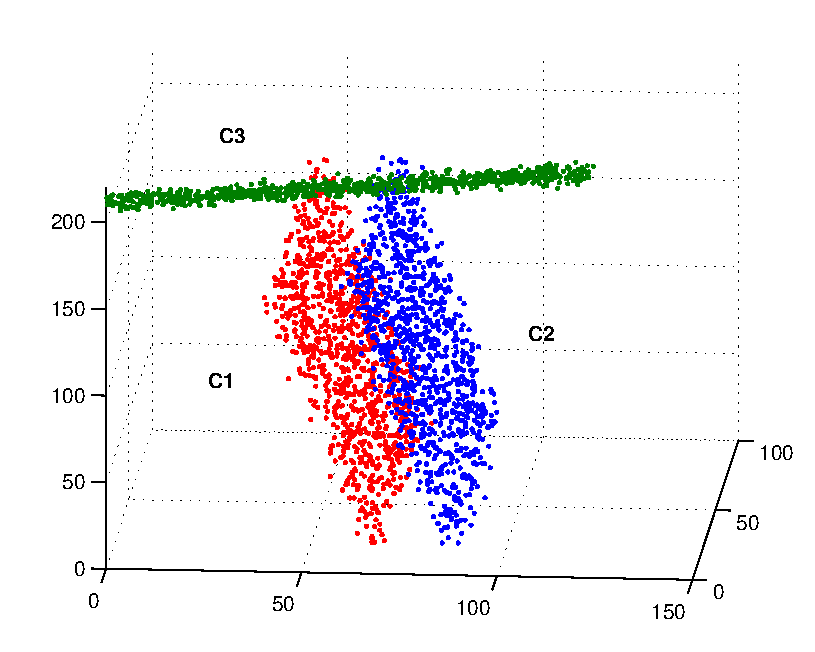
\includegraphics[width=3.5in]{img/LmDemo}
\IfClass{IEEEtran}{\vspace*{-25pt}}{}
\caption{Example of points forming three linear manifold clusters.
The green cluster is one dimensional. The blue and red clusters are
two dimensional and parallel \cite{Haralick:2007rt}.}
\label{fig:lm-demo}
\end{figure}

Linear manifold clusters \cite{Haralick:2007rt} can be found by a stochastic
search procedure, beginning with the one dimensional linear manifold clusters
and proceeding to higher dimensional clusters. A one dimensional linear manifold
is determined by two points. The stochastic search samples two points from
the data set, forms the manifold, and then the distances from all points to the
discovered manifold are calculated. If the manifold is indeed one that has many
data points close to it, the distance histogram will have a peak close to 0
distance followed by a valley and then a rise to a long fat tail or another peak
far from the origin, see Fig.~\ref{fig:dist-hist-sep}.

\begin{figure}[h]
\centering
\IfClass{IEEEtran}{
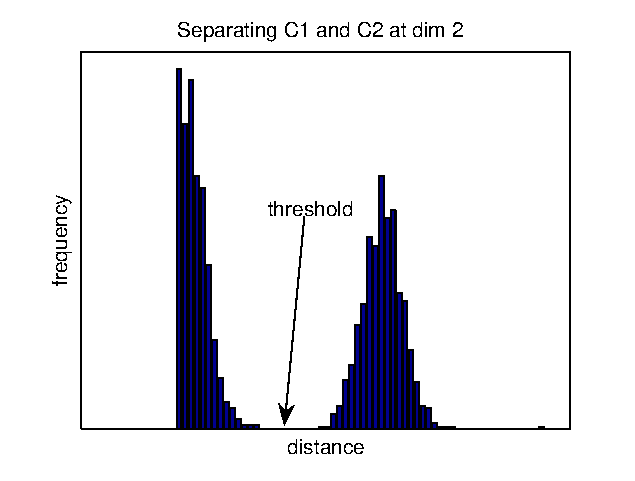
\includegraphics[width=3.5in, height=2.2in]{img/C1C2sepD2}
\vspace*{-30pt}
}{
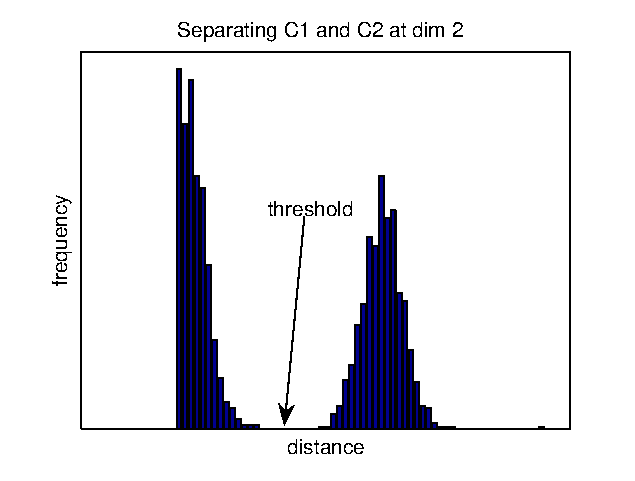
\includegraphics[width=3.5in]{img/C1C2sepD2}
}
\caption{Example of a distance to manifold histogram that shows that
a linear manifold cluster can be formed from the test manifold \cite{Haralick:2007rt}.}
\label{fig:dist-hist-sep}
\end{figure}

If this happens, then a suitable threshold can be found that separates
the data points that are near to the manifold from those data points that are
far away from the manifold. The data points that are near the manifold are
collected together and are used to make a good statistical estimate for
the manifold basis and offset. The manifold basis is given by the first
$M$ principal components of the cluster data points, where $M$  is the dimension
of the manifold. The offset can simply be the mean of the data points in
the cluster. Manifolds that do not have the right shaped distance to manifold
histograms do not get the chance to form clusters.

\IfClass{IEEEtran}{}{
Figure~\ref{fig:dist-hist-nosep} illustrates a distance to manifold histogram in
which the test manifold cannot be used to form a linear manifold cluster.
\begin{figure}[h]
\centering
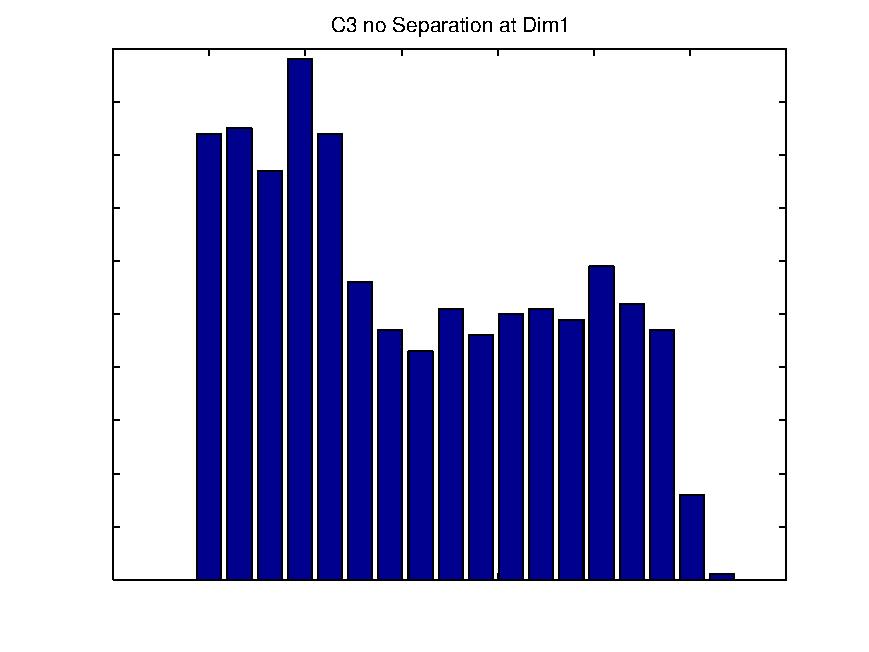
\includegraphics[width=3.5in]{img/C3nosepD1}
\caption{Illustrates a distance to manifold histogram in which the test manifold
cannot be used to form a linear manifold cluster}
\label{fig:dist-hist-nosep}
\end{figure}
}

Our linear manifold clusters must satisfy two criteria. First, the goodness of
a separation between the mode near zero and rest of the point-to-manifold
distance histogram modes should be larger then the user specified.
This criterion is fully explained in \cite{Haralick:2007rt}.
Second, the cluster compression ratio, defined as the ratio between
the linear manifold cluster description length and the uncompressed description length of the cluster, should be larger then the user defined threshold.
This criterion, in effect, acts as an internal validation the cluster
goodness-of-fit, and it is a new addition to the algorithm described
in \cite{Haralick:2007rt}.

\IfClass{IEEEtran}{}{
We extend MDL principle, so it would allow us some inexactness in
describing manifold cluster data, which can be viewed as a lossy data compression,
without loss of general understandability of the cluster structure.
%
The fundamental idea behind the MDL principle is that every regularity in
the data can be used to compress the data \cite{Grunwald:2007Gr}.
Such a description should always uniquely specify the data it describes -
hence given a description or encoding of a particular data sequence, we should
always be able to fully reconstruct data.
}
       % Linear Manifold Clustering
% -*- root: inexact_mdl_lmc.tex -*-
\section{MDL Linear Manifold Cluster Description}
\label{sc:mdl-lmclus}
\IfClass{IEEEtran}{}{
We use the MDL principle to determine the number of bits required to describe the
points of a candidate linear manifold cluster with a controlled total squared error.
If this number of bits is not sufficiently smaller than the number of bits to
represent in their raw form the points associated with the candidate linear
manifold cluster, the candidate linear manifold cluster is rejected.
}
First we determine the number of bits it takes to encode the translational
offset of the linear manifold and then the orthonormal basis vectors
spanning the linear manifold. Then we determine the number of bits it takes
to encode the points of the candidate linear manifold cluster to
within a given squared error.

Let $X = \{x_j \in \mathbb{R}^N | \; j = 1, \dots, J \} $ be the points
associated with the $M$-dimensional linear manifold cluster $\mathcal{M}$.
It is described by a set of orthonormal basis vectors, that span the linear
manifold, $B = \{b_m \in \mathbb{R}^N | m = 1, \dots, M \}$ and
a translation vector $\mu \in \mathbb{R}^N$.

\paragraph{Model Encoding}
The encoding of the translation vector $\mu$ requires $N$ numbers.

To represent any vector $x$, after its translation, we need the basis vectors
spanning the manifold and we need the basis vectors orthogonal to the manifold.
From the basis vectors spanning the manifold we can determine the relative
coordinates of the orthogonal projection of $x$ to the manifold and from
the basis vectors spanning the orthogonal complement space, we can determine
the orthogonal projection of $x$ to the complement space.

Since the basis vectors of the linear manifold and its orthogonal compliment
space are orthonormal, we can represent the basis vectors in less than $N^2$
numbers. We can use a decoding schema that uses the orthonormal constraints in
recovering the $N$ basis vectors. Each basis vector has norm 1. This constitutes
$N$ constraints. The orthonormality constraints specify another $N(N-1)/2$
constraints. The total number of orthonormality constraints is then $N(N+1)/2$.

To describe the linear manifold requires $N$ numbers for the offset of
the manifold from the origin plus $N^2 - N(N+1)/2$ numbers for basis vectors.
Letting $P_m$ be the number of bits used for encoding each component of
the offset and each of the numbers required to calculate the basis vectors.
Then the total number of bits, $L(H)$, required to specify the structure of
a linear manifold and its orthogonal complement space is

\begin{equation} \label{eq:mdl-lmc-model}
L(H) = P_m [ N + N(N-1)/2) ] = P_m N(N+1)/2
\end{equation}

\paragraph{Data Encoding}

Let $B^{N\times M}$ be a matrix whose columns are the orthonormal basis vectors
spanning the linear manifold. Then the relative coordinates of the orthogonal
projection of a vector $x-\mu$ to the manifold is given by $B^T (x-\mu)$.
This is a vector of dimension $M\times 1$. Each of the $M$ components of this
vector will be encoded with $P_d$ bits.
\IfClass{IEEEtran}{}
{
Hence the encoding requires $P_d M$ bits.
Since the offset $\mu$ lies in $col(B)$, $BB^T \mu = \mu$ and
the reconstruction of that part of $x$ that lies on the manifold is then given
by $\mu+B(B^T(x-\mu))$.
}

Let $\bar B^{N\times N-M}$ be a matrix whose columns are the basis vectors
spanning the orthogonal complement space. The relative coordinates of
the orthogonal projection of a vector $x-\mu$ to the complement space of
the manifold is given by $\bar B^T (x-\mu)$. This is a vector having $N-M$
components. The reconstruction of that part of $x$ that lies in the orthogonal
complement space is given by $\bar B(\bar B^T(x-\mu))$.

The total number of bits required to encode data $D$ given a model $H$ is
\begin{equation} \label{eq:mdl-lmc-data}
L(D|H) = J [P_d M + S(\varepsilon)]
\end{equation}
where $J$ is number of points in the linear manifold cluster, $S$ is the entropy
of the distribution of cluster points, in the orthogonal compliment subspace to
the linear manifold of the cluster, calculated to be correct within
the fitting error $\varepsilon$.

We assume that each of the $K=N-M$ components of that part of $x$ that lies in
the orthogonal complement space is uniformly distributed, but that the interval
of the uniform distribution is different for each component. For component $k$,
we let the uniform distribution be defined on the interval $[-A_k/2,A_k/2]$.
We will quantize the interval $[-A_k/2,A_k/2]$ into $N_k$ equal length
quantizing intervals and encode component $k$ by the index of the quantizing
interval into which it lies.
Since the intervals are all equal length, knowing the index of the subinterval
into which a value falls, permits the value of to be approximated by the mean
of the subinterval into which it falls. The squared error is then the variance
of a uniform distribution over the subinterval.

\IfClass{IEEEtran}{
Set the log of the total number of quantized choices in
the $K$-dimensional space equal to a given $C =\sum_{k=1}^K \log N_k$.
}
{
The variance of a uniform over an interval of length $L$ is
$$
\frac{1}{12}L^2
$$
%
The interval $[-A_k/2,A_k/2]$ has length $A_k$. If this interval is divided to
$N_k$ subintervals, the variance of each subinterval is then
$$
V_k=\frac{1}{12}\left(\frac{A_k}{N_k}\right)^2
$$
%
The meaning of this variance is that regardless of the actual value of
the $k^{th}$ component, the squared error arising from using the middle of
the interval to which it belongs is $V_k$.
%
The variance over all the $K$ quantized components is then
%
$$
\frac{1}{12}\sum_{k=1}^K \left(\frac{A_k}{N_k}\right)^2
$$
%
The optimal quantizing problem is to minimize the total error
$$
E^2=\frac{1}{12}\sum_{k=1}^K \left(\frac{A_k}{N_k}\right)^2
$$
by choice of the optimal values for $N_1,\ldots,N_K$ subject to
the constraint that the log of the total number of quantized choices in
the $K$-dimensional space is equal to a given $C$.
$$
\sum_{k=1}^K \log N_k=C
$$
%
Define
$$
\epsilon^2=\sum_{k=1}^K \left(\frac{A_k}{N_k}\right)^2+\lambda\left(\sum_{k=1}^K \log N_k-C\right)
$$
%
\begin{eqnarray*}
\frac{\partial \epsilon^2}{\partial N_k}&=&A_k^2(-2)N_k^{-3}+\lambda\frac{1}{N_k}\\
0&=&A_k^2(-2)N_k^{-3}+\lambda\frac{1}{N_k}\\
2A_k^2 N_k^{-2}&=&\lambda\\
N_k^2&=&\frac{2A_k^2}{\lambda}\\
N_k&=&\frac{2^{\frac{1}{2}}A_k}{\lambda^{\frac{1}{2}}}\\
\log N_k&=&\frac{1}{2}\log 2+ \log A_k -\frac{1}{2}\log \lambda
\end{eqnarray*}
This relation permits $\lambda$ to be determined in terms of $C$ and $A_1,\ldots,A_K$\bigskip
\begin{eqnarray*}
C=\sum_{k=1}^K \log N_k&=& \sum_{k=1}^K\left( \frac{1}{2}\log 2+ \log A_k -\frac{1}{2}\log \lambda\right)\\
-\frac{K}{2}\log\lambda&=&C-\frac{K}{2}\log 2-\sum_{k=1}^K\log A_k\\
-\frac{1}{2}\log\lambda&=&\frac{C}{K}-\frac{1}{2}\log 2 -\frac{1}{K}\sum_{k=1}^K \log A_k
\end{eqnarray*}
Substituting the expression for $-\frac{1}{2}\log \lambda$ into the expression
for $\log N_k$ will permit us to determine $N_k$ in terms of $C$ and $A_1,\ldots,A_K$.
\begin{eqnarray*}
\log N_k&=&\frac{1}{2}\log 2+ \log A_k+\frac{C}{K}-\frac{1}{2}\log 2 -\frac{1}{K}\sum_{j=1}^K \log A_j\\
&=&\log A_k+\frac{C}{K}-\frac{1}{K}\sum_{j=1}^K \log A_j
\end{eqnarray*}
}

From this it follows that the integer value of $N_k$ can be taken to be
the smallest integer $N_k$ satisfying
\begin{equation}\label{eq:quant-intervals}
N_k(C) = \lceil A_k e^{(C-\sum_{j=1}^K \log A_j)/K} \rceil
\end{equation}

The interval lengths $A_1,\ldots,A_K$ are given and fixed.
The values of $N_1,\ldots,N_K$ are each dependent on the value of $C$.
So we can write the squared error $E^2$ as the variance of a uniform
distribution over all subintervals of the $K$ quantized components,

\begin{eqnarray}\label{eq:sq-quant-error}
E^2(C)=\frac{1}{12}\sum_{k=1}^K \left(\frac{A_k}{N_k(C)}\right)^2
\end{eqnarray}

If we operate under the protocol that the quantizing must be done fine enough,
such that for the user specified quantization error bound $\varepsilon$,
the value of $C$ is small enough to satisfy
\begin{equation}\label{eq:error-condition}
 E^2(C) < \varepsilon^2
\end{equation}

\IfClass{IEEEtran}{}{
If the maximum number of intervals $N_k$ is limited by the maximum integer
value available for particular computational architecture, $N_{max}$. For 32-bit
architecture, $N_{max}$ is $2^{32}$ .
%
Given $N_{max}$ and length of intervals $A_k \geq 1$, we can calculate the upper
bound of the value $C$ as follows
%
\begin{eqnarray*}
\log N_{max} &=& \log A_k+\frac{C}{K}-\frac{1}{K}\sum_{j=1}^K \log A_j \\
C &=& \min_{k} \left(K \log\frac{N_{max}}{A_k} +\sum_{j=1}^K \log A_j\right)
\end{eqnarray*}
%
For the lower bound of the value $C$, we use only one quantization interval in
(\ref{eq:quant-intervals}) which results in
%
\begin{eqnarray*}
\log 1 &=& \log A_k+\frac{C}{K}-\frac{1}{K}\sum_{j=1}^K \log A_j \\
C &=& \min_{k} \left(K \log \frac{1}{A_k} +\sum_{j=1}^K \log A_j \right)
\end{eqnarray*}
}
then is not hard to show that the value $C$ is defined over the interval
\[
% \min_k \left(K [0,\log N_{max}] - \log A_k + \sum_{j=1}^K \log A_j \right)
\left[ 0, K \log N_{max} \right] + \sum_{j=1}^K \log A_j - \min_k \log A_k
\]

We can find the optimal number of quantization intervals $N_k$ with a given user
defined precision value $\varepsilon$ by performing a search for appropriate
value of $C$ in the above interval such that it would satisfy
condition \eqref{eq:error-condition}.

Given the value $C$ that satisfies \eqref{eq:error-condition}, we can calculate
the number of bits required to encode the position of the cluster point in
the orthogonal complement space of the linear manifold cluster. The value $C$
corresponds to the entropy $S$ of a distribution of cluster points in
the orthogonal compliment space, that is required in \eqref{eq:mdl-lmc-data}.
Since the logarithms are to base $e$, $C$ does not have the meaning of bits.
But
\IfClass{IEEEtran}{}{
\begin{equation*}
C\log_2 e = \sum_{k=1}^K \log_2 N_k
\end{equation*}
}
\begin{equation*}
\frac{C}{\log 2} = \sum_{k=1}^K \log_2 N_k
\end{equation*}
does have the meaning of bits.

\IfClass{IEEEtran}{}{
Another approach would be calculation of the the empirical entropy of
the points' coordinate distribution in the orthogonal compliment space.
Given the number of quantization intervals $N_k$, we can calculate
the empirical entropy of the point distribution in the orthogonal complement
space of the linear manifold cluster as
\begin{equation}\label{eq:ocs-point-entropy}
S = -\sum_{k=1}^{K} \sum_{j=1}^{N_k} p_{kj} \log p_{kj}
\end{equation}
where $p_{kj}$ is a probability that the point is located in the bin $N_j$ of
the interval $A_k$ for $k$th dimension of the orthogonal complement space.
%
Orthogonal complement projection associates directions where points extend
orthogonality from the cluster support defined by the cluster linear manifold.
In order to calculate orthogonal complement projection, we calculate principal
components of the cluster points through the singular value decomposition, as
$X = U \Sigma V^T$.
The first $M$ columns of $U$ provide vectors that span the linear manifold,
defined as the columns of matrix $B$, and last $N-M$ vectors provide vectors
that span orthogonal complement subspace, for the cluster linear manifold.
The columns of matrix $B^\perp$ are created from the last $N-M$ columns of
matrix $U$. Thus, an orthogonal complement projection of cluster points:
$d = {B^\perp}^T x$ for $x \in X$. The given projected points are used
in (\ref{eq:ocs-point-entropy}) for determining the value of $S$.
%
For each of $N-M$ dimensions, the histogram with $N_k$ bins for orthogonally
projected data points is constructed to determine probability, $p_{kj}$, of
the points existence in the $N_j$ interval, for calculating (\ref{eq:ocs-point-entropy}),
the value of entropy $S$ with the specified error value $\varepsilon$.
}

Using the above descriptions of model \eqref{eq:mdl-lmc-model} and
data message \eqref{eq:mdl-lmc-data} length, the total length of
the message for linear manifold cluster (LMC) is calculated as
\begin{equation} \label{eq:mdl-lmc-final}
L(\varepsilon) = P_m N(N+1)/2 + J(P_d M  + S(\varepsilon))
\end{equation}

From (\ref{eq:mdl-lmc-final}), we can see that two factors affect description
length - the precision constants and the entropy.
If simple models of the linear manifold cluster are favored then the entropy and
the precision parameters should be proportionate. It would allow stable growth
of the description length with respect to the size and the dimensionality of
the linear manifold cluster.

If we want to determine a optimal clustering parameters, it is important
to use the encoding that does not calculate the data points in the clusters,
but the distribution of the data points in each of the clusters.
The difference is this: to characterize the data points in the cluster,
the number of bits required will increase with the number of data points.
However the characterization of the distribution does not depend on
the particular number of points: it depends on representing the various
parameters of each of the clusters so that from the representation a sample of
data points can be generated that would be indistinguishable from
the original sample. Or to say this another way, the clustering is
to characterize the population from which the observed data has been sampled.

We use model encoding schema as given in \eqref{eq:mdl-lmc-model}, as for data
encoding is determined based on a the spread of the data on the manifold and
as well in the orthogonal complement space.

For an $M$-dimensional manifold, we can use the first $M$ eigenvalues as the
variance of the spread on the manifold. Since this is from a principal
components, the covariance matrix is diagonal. The distribution of the data on
the manifold, then can be described as a Normal distribution with the mean
being given by the translation vector and the covariance matrix being
diagonal with the diagonal entries coming from the first $M$ eigenvalues
of the principal components.

For the orthogonal complement subspace, we assume a more general model that
allows for a description that is accurate to within a user specified error.
We model the distribution based on the quantization of orthogonal complement
subspace $N-M$ dimensions. Each of these dimensions has an observed minimum
value, a maximum value and number of quantized bins as determined by the entropy
calculation and the user specified error. As well, each of the bins has
a probability. To generate points in the orthogonal complement space,
for each of its dimensions, we can choose a bin in accordance with the bin
probabilities and within a bin choose a value uniformly distributed between
the quantizing boundaries of the bin.

The $M$ coordinates generated from the manifold and the $N-M$ coordinates chosen
from the orthogonal complement space then can be used as coefficients of their
respective basis vectors to produce a vector in the $N$-dimensional space.

\IfClass{IEEEtran}{}{
The number of parameters to specify an $M$ dimensional manifold data is then
%
\begin{eqnarray*}
M + \sum_{m=M+1}^N Q_m+1+Q_m& =& M + (N - M) + 2\sum_{m=M+1}^N Q_m
\end{eqnarray*}
%
where $Q_m$ is the number of quantized levels for orthogonal complement
dimension $m$, the plus 1 is because to have $Q_m$ quantized levels there
needs to be $Q_m+1$ boundaries and the second $Q_m$ is because each
quantized level has to have a probability.
}

\begin{equation} \label{eq:mdl-lmc-data-pop}
L(D|H) = P_d \left(N+2\sum_{m=M+1}^N Q_{m} \right)
\end{equation}
where $Q_m$ is the number of quantized levels for orthogonal complement
dimension $m$.

We can assume that because of the MDL in the clustering, regardless of
the value of the input parameters that the user set, the clustering gives an
appropriate characterization of the distribution of the population from which
the observed data set was sampled. The best characterization of the population
is the characterization that has fewest bits and calculated as

\begin{equation} \label{eq:mdl-lmc-final-pop}
L(\varepsilon) = P_m N(N+1)/2 + P_d \left(N+2\sum_{m=M+1}^N Q_{m}(\varepsilon) \right)
\end{equation}
   % MDL Linear Manifold Cluster
\section{Results} \label{sc:results}

\ifIEEEtran
\else
We perform series of experiments to test the MDL description for the linear
manifold (LM) cluster described in section~\ref{sc:mdl-lmclus}.
Our first experiments are parametric experiments to illustrate the effect of
the number of precision bits carried and to understand the effect of
the error bound. The second experiment illustrates the results of the MDL linear
manifold clustering operating on different data sets.




First, we looked at how the quantization error $\varepsilon$ affects resulting
value of the MDL LM cluster description. We generated a 1D linear
manifold cluster, composed of 1000 points, in 2D Euclidean space where
points' coordinates where drawn from zero-mean normal distribution, independent
for every coordinate dimension.
In order to archive cluster shape compatible with 1D linear manifold, we used
different variances for each coordinate dimension. For $x$ coordinate,
the variance of the normal distribution is $\sigma_x = 1$ and for $y$ coordinate
$\sigma_y = 0.1$. Such cluster generation procedure creates a linear manifold
cluster, see Fig.~\ref{fig:lmc}, which is bounded in $x \in [-3;3]$ and
$y \in [-0.33;0.33]$.

\begin{figure}[ht]
\center
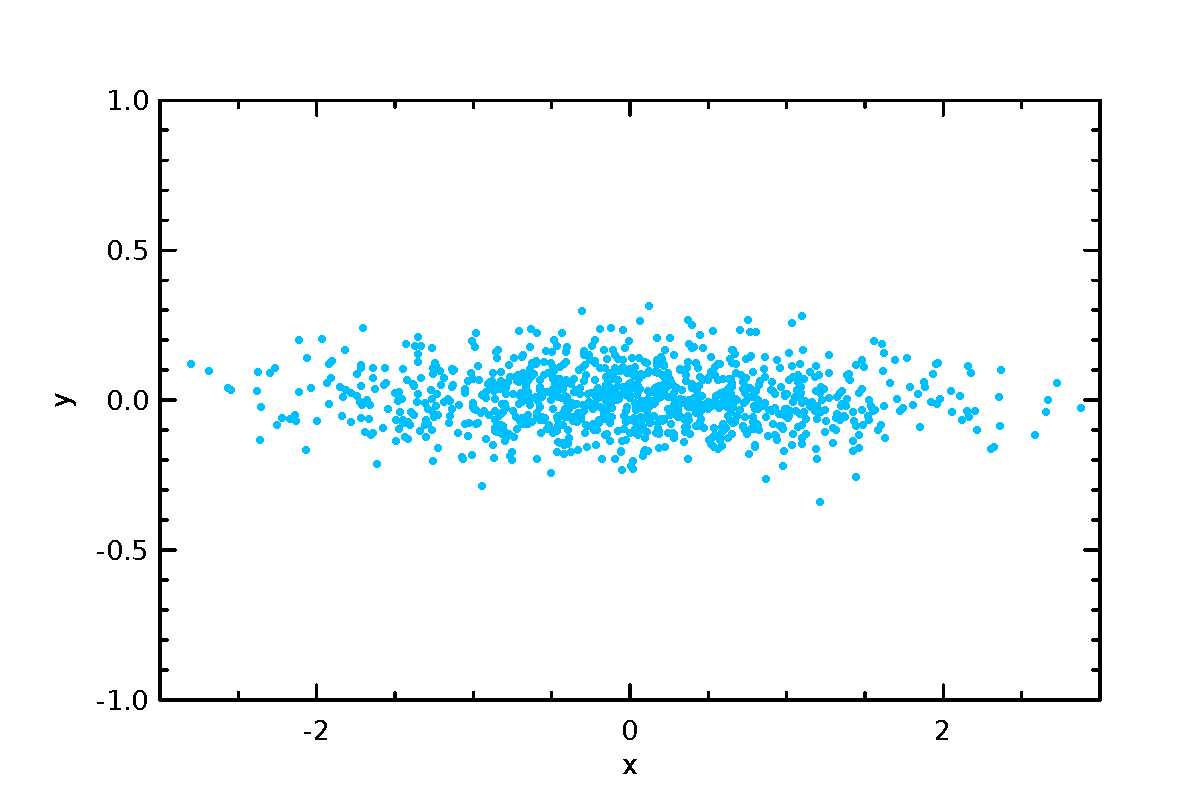
\includegraphics[width=3.5in]{img/results_lmc_1.pdf}
\caption{1D linear manifold cluster in 2D space}
\label{fig:lmc}
\end{figure}



For each quantization error $\varepsilon$, in range of values from $10^{-1}$ to
$10^{-8}$, we generate 100 LM clusters following above generation procedure and
calculate an average cluster MDL value and its 95\% confidence interval,
see Fig.~\ref{fig:mdl-exp1}. It is important to mention, there are two more
parameters involved in calculation of the cluster MDL value - model and data
encoding precision constants. These constants were set to 24 and 16 bits
accordingly.

% % Compose plots with subfigures (remove all figures fig:mdl-exp[1-2])
% \begin{figure}[ht]
% \hspace*{-60pt}
% \subfigure[]{
%     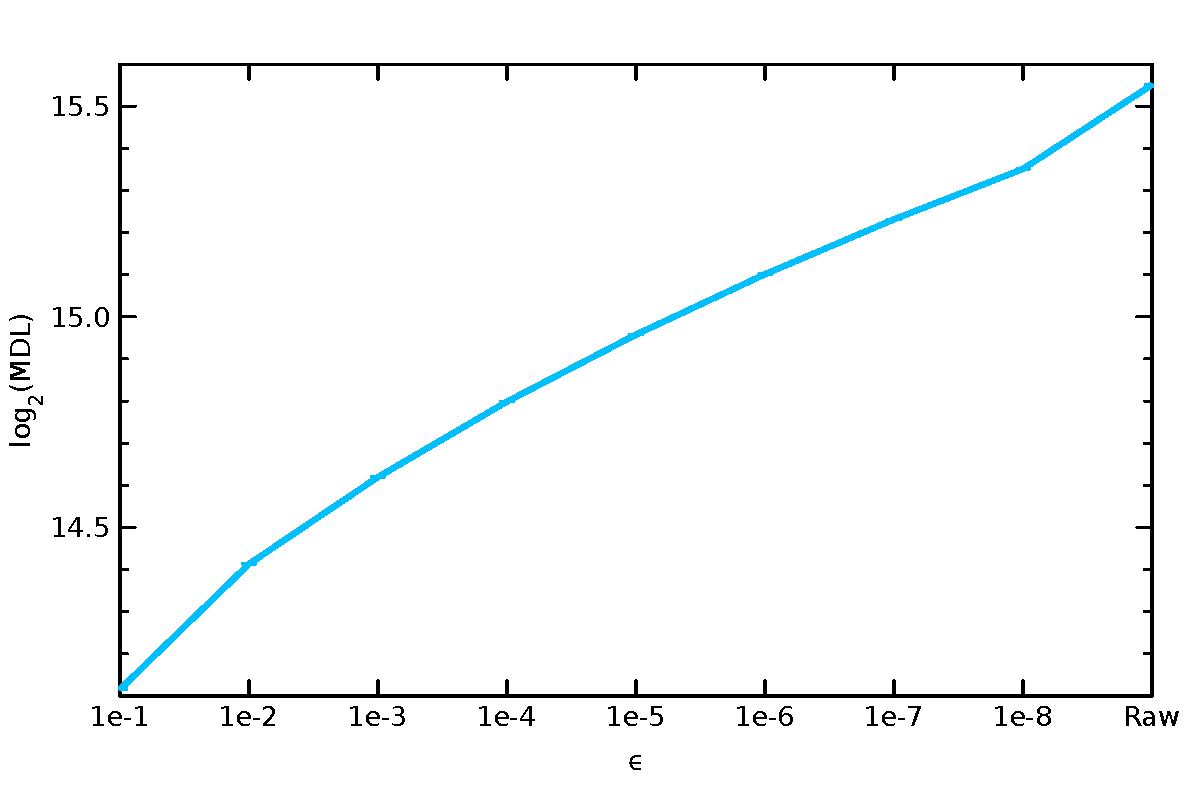
\includegraphics[width=3.5in]{img/results_mdl-exp1_1.pdf}
%    \label{fig:mdl-exp1}}
% \subfigure[]{
%     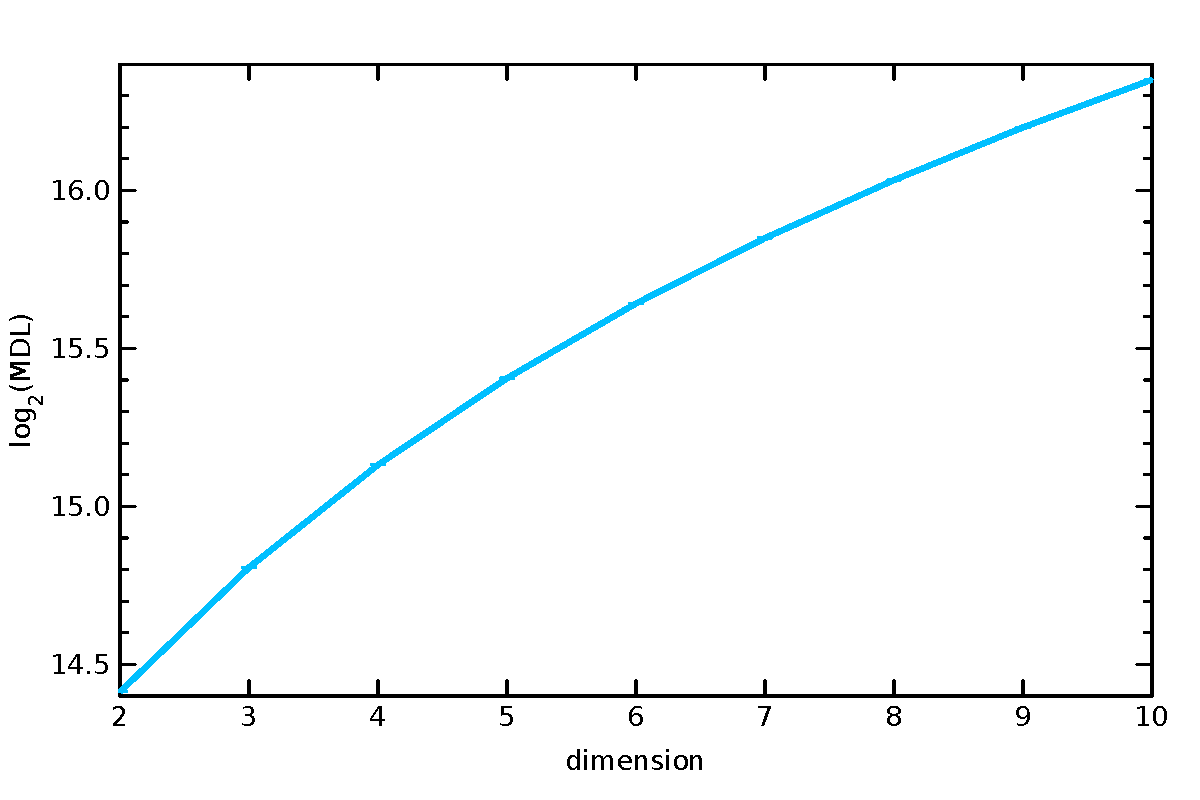
\includegraphics[width=3.5in]{img/results_mdl-exp2_1.pdf}
%     \label{fig:mdl-exp2}}
% \caption{
%     \subref{fig:mdl-exp1} MDL value of 1D LM cluster, in 2D space, calculated with quantization error \textepsilon; ``Raw'' value corresponds to the encoding without a model.
%     \subref{fig:mdl-exp2} MDL value of 1D LM cluster generated in a space of dimension from 2 to 10.
% }
% \end{figure}

\begin{figure}[ht]
\center
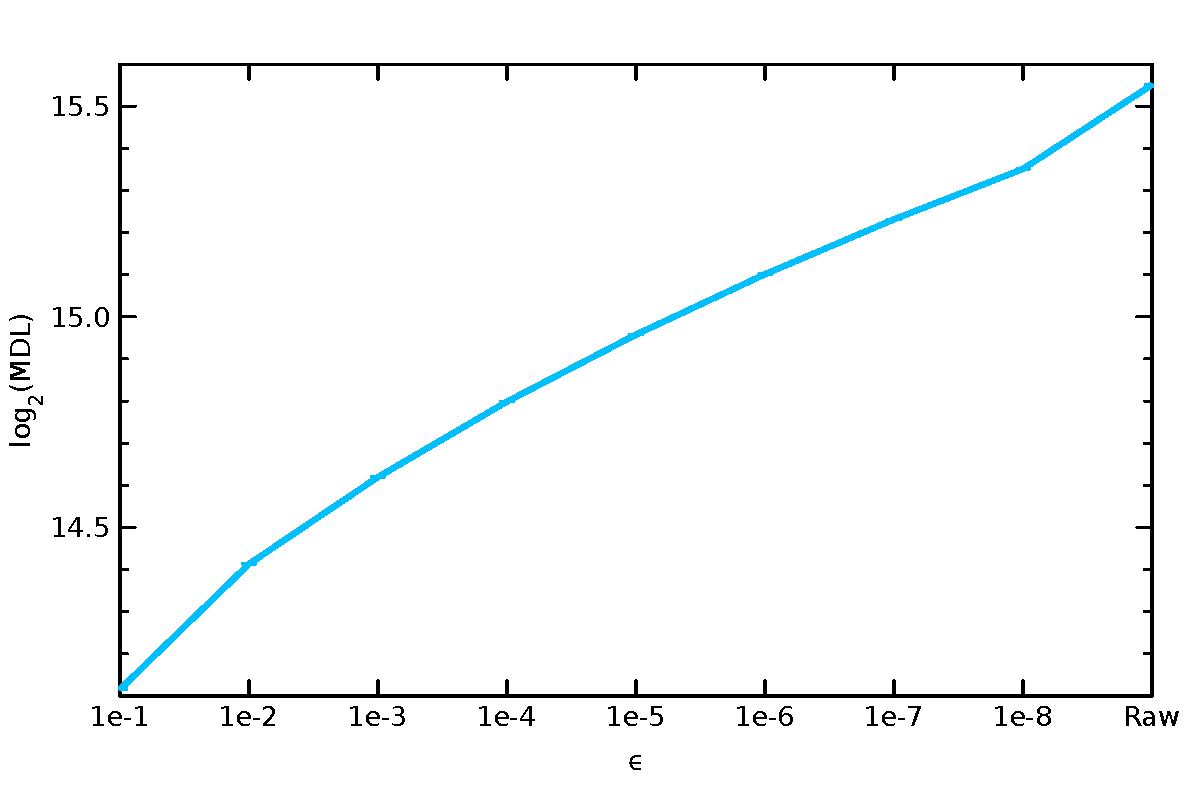
\includegraphics[width=4in]{img/results_mdl-exp1_1.pdf}
\caption{MDL value of 1D linear manifold cluster, in 2D space, calculated with quantization error \textepsilon. ``Raw'' value corresponds to the encoding without a model.}
\label{fig:mdl-exp1}
\end{figure}



As expected, while the quantization error decreased, there was a more
precise encoding of point distribution in the orthogonal complement space of the
cluster manifold and  the corresponding MDL value of the LM cluster increased
up to the maximum possible value of uncompressed raw encoding.
\bigskip
%
Next, we investigated dependency of the MDL value on the LM cluster dimension. We
calculated MDL values of a 1D linear manifold cluster in full space of dimension
from 2 to 10. In order to generate 1D LM cluster for high dimensional spaces,
we used same methodology as with a 2D space, first coordinate was generated from
normal distribution with variance 1.0, the rest of the coordinates were drawn
from normal distribution with variance 0.1. We used same encoding constants as
in previous experiment, and the value of quantization error was set to 0.01.

As we expected, the MDL value of the 1D LM cluster would increase with number of
space dimensions. This is shown in Fig.~\ref{fig:mdl-exp2}.
\bigskip

\begin{figure}[ht]
\center
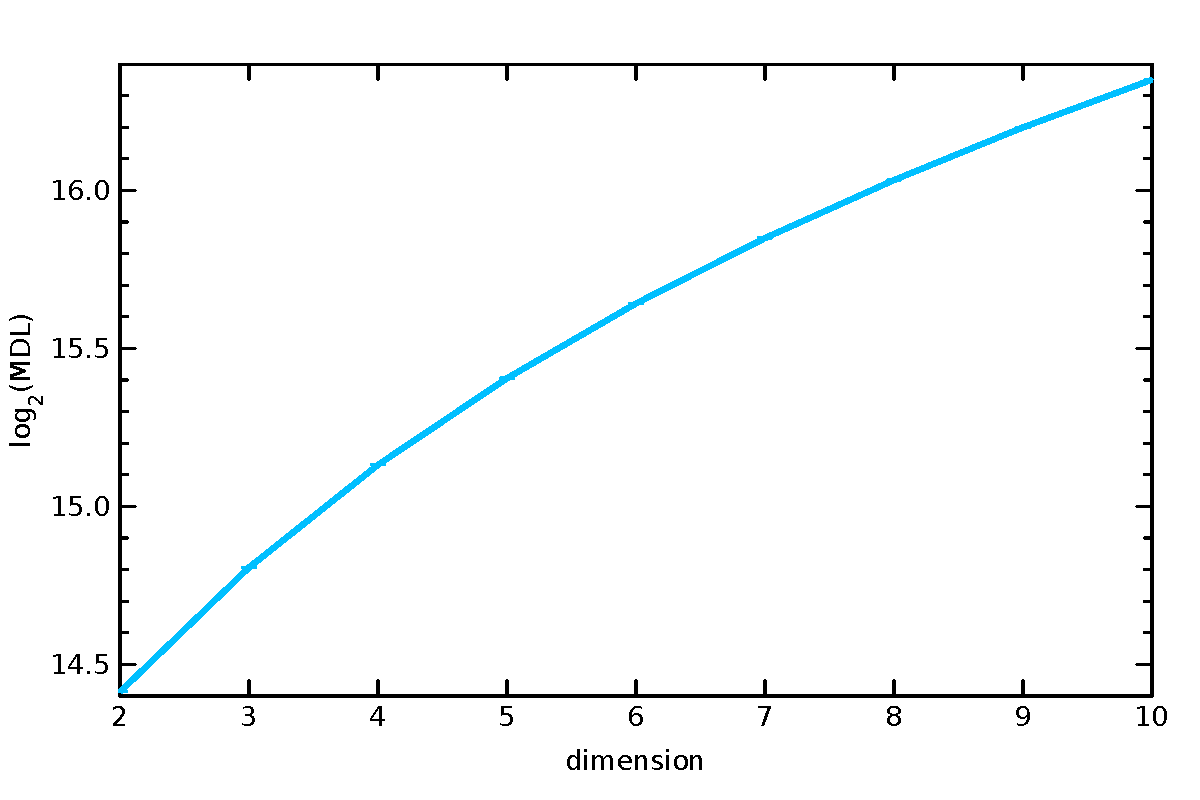
\includegraphics[width=4in]{img/results_mdl-exp2_1.pdf}
\caption{MDL value of 1D linear manifold cluster generated in a space of dimension from 2 to 10.}
\label{fig:mdl-exp2}
\end{figure}



Also, we investigated the dependency of the MDL value of LM cluster as
the encoding precision constants changes. In above experiments, we use values of
24 and 16 for the model and data encoding precision constants. We varied these
pair of constant for calculation of MDL value for a 1D LM cluster in 2D space.


% % Compose plots with subfigures (remove all figures fig:mdl-exp[3-4])
% \begin{figure}[ht]
% \hspace*{-50pt}
% \subfigure[]{
%     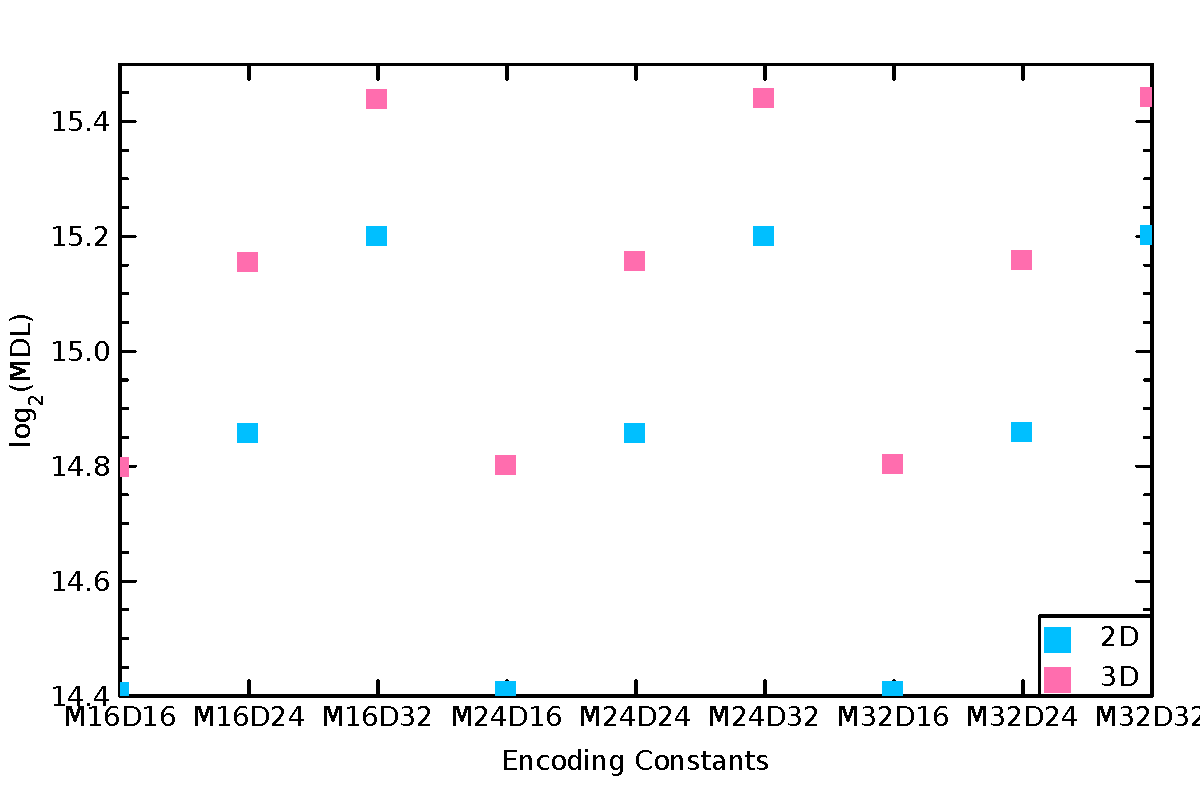
\includegraphics[width=3.5in]{img/results_mdl-exp3_1.pdf}
%     \label{fig:mdl-exp3}}
% \subfigure[]{
%     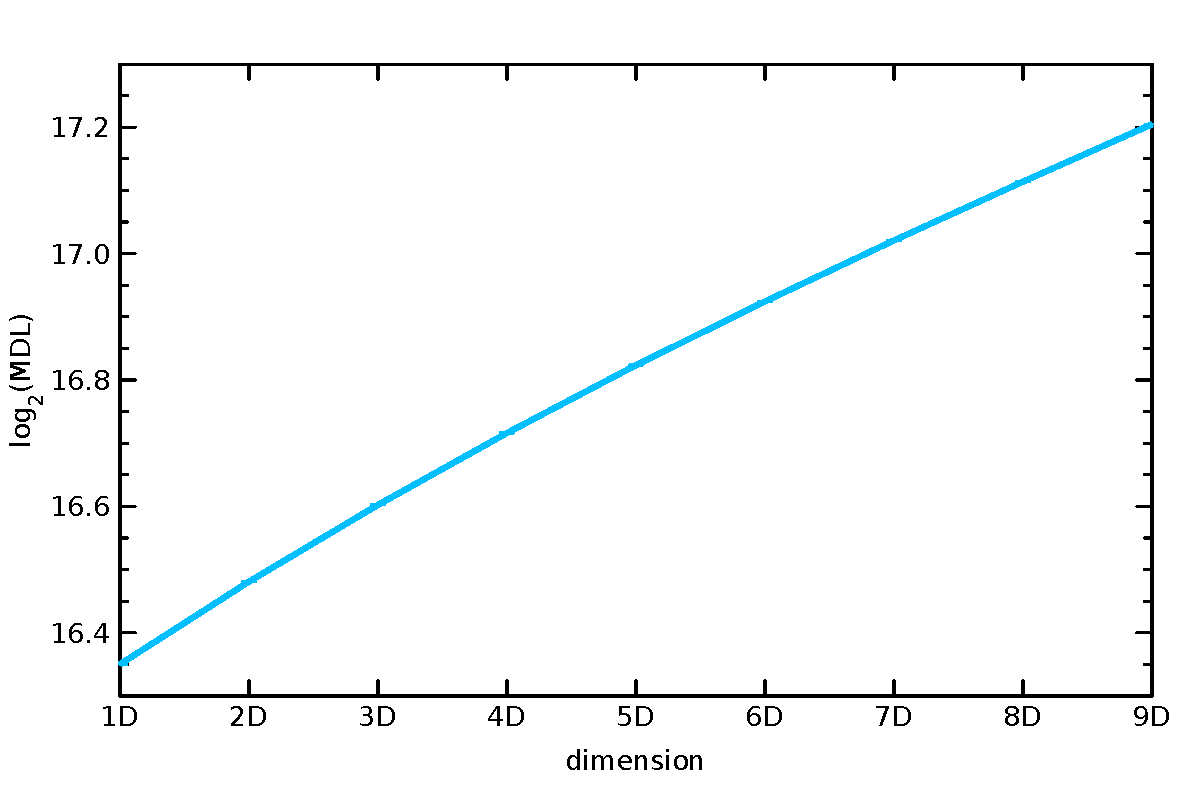
\includegraphics[width=3.5in]{img/results_mdl-exp4_1.pdf}
%     \label{fig:mdl-exp4}}
% \caption{
%     \subref{fig:mdl-exp3} MDL value of 1D LM cluster in 2D space w.r.t. encoding constants (\emph{EConst} axis shows values of encoding constants as \emph{m[I]d[J]} where $I$ is model constant value and $J$ is data constant value).
%     \subref{fig:mdl-exp4} MDL values of LM clusters with dimensions from 1 to 9 in 10D space.
% }
% \end{figure}

\begin{figure}[H]
\center
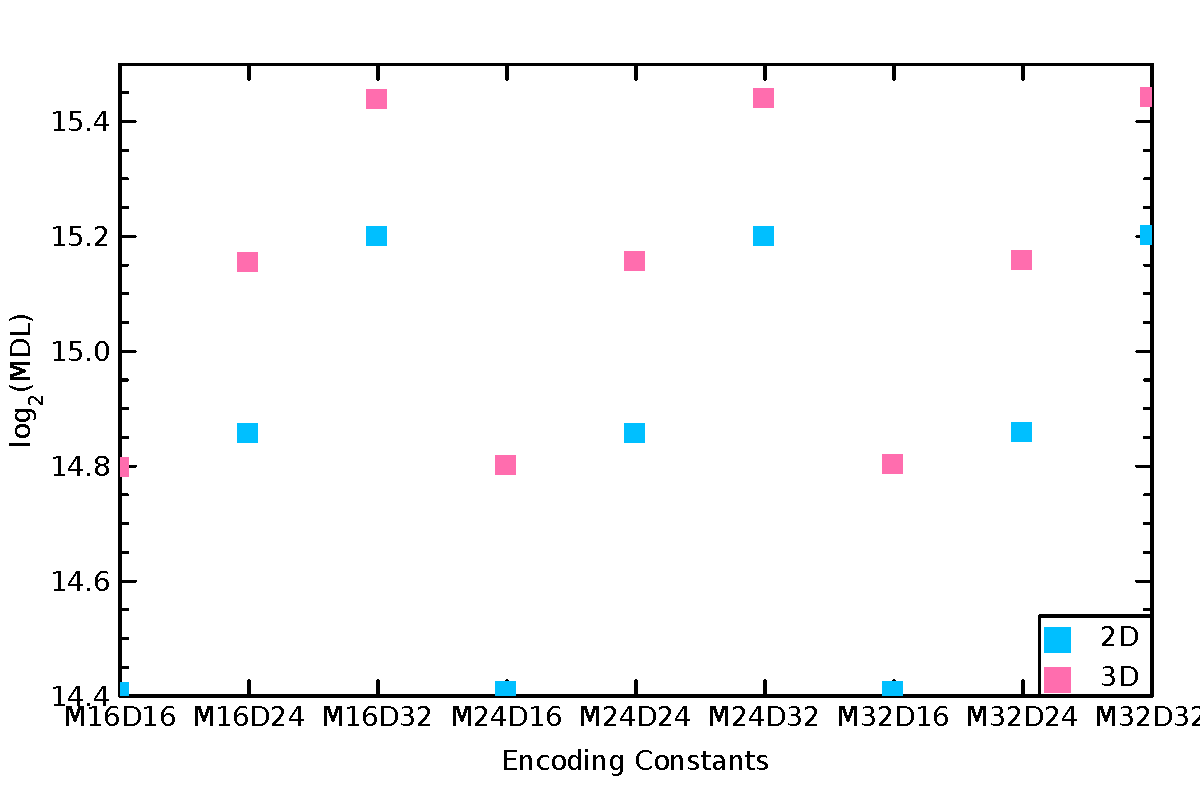
\includegraphics[width=4in]{img/results_mdl-exp3_1.pdf}
\caption{MDL value of 1D linear manifold cluster in 2D space w.r.t. encoding constants (\emph{Encoding Constants} axis shows values of encoding constants as \emph{M[I]D[J]} where $I$ is model constant value and $J$ is data constant value).}
\label{fig:mdl-exp3}
\end{figure}



Fig.~\ref{fig:mdl-exp3} shows that the model encoding constant does not
contribute much to overall value of the cluster MDL. For 1D linear manifolds in
2D and 3D space, the main factor which affects the resulting MDL value is
the data encoding precision constants.
\bigskip
\fi

% LM type: Compare 1D and 2D LM cluster in 3D
\ifIEEEtran
\else
The following experiment allows us to determine how the dimensionality of
the LM cluster affects the calculation of its MDL value. We create multiple
linear manifolds with increasing dimension in a 10 dimensional space. LM cluster
generation is done in a standard way: generate coordinate values of the cluster
points from a normal distribution. For a primary dimension of the LM cluster,
the variance is 1.0, and for dimensions in the orthogonal complement to
the linear manifold, the variance is set to 0.1. The encoding constants,
model and data, are 24 and 16. The quantization error bound is set to 0.01.

\begin{figure}[H]
\center
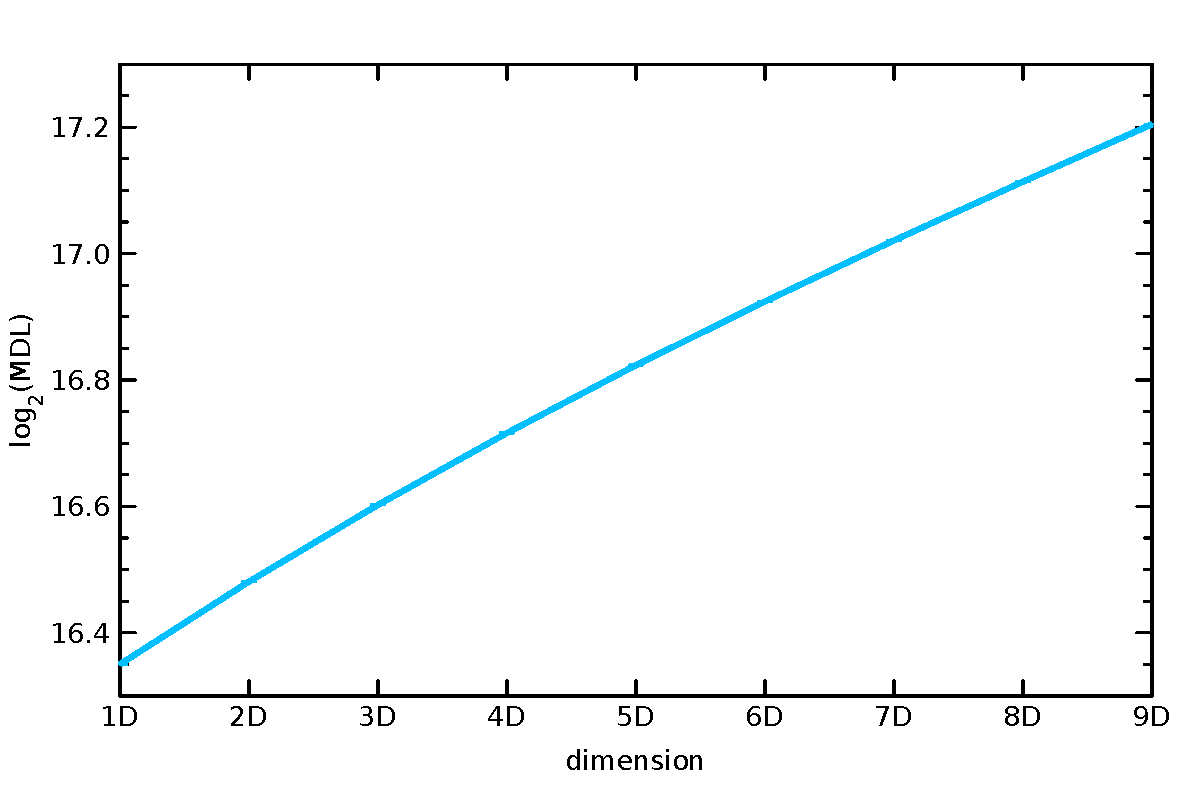
\includegraphics[width=4in]{img/results_mdl-exp4_1.pdf}
\caption{MDL values of LM clusters with dimensions from 1 to 9 in 10D space.}
\label{fig:mdl-exp4}
\end{figure}



Fig.~\ref{fig:mdl-exp4} shows expected linear growth of the MDL value with
the manifold dimensionality which is reflected in first term
of (\ref{eq:mdl-lmc-data}). More coordinates are encoded with constant factor
$P_d$ which is overpowering entropy term of coordinates in the orthogonal
complement space of the LM cluster.
\fi

% Take a J-dimensional manifold cluster and calculate MDL as if cluster dim != J
Finally, we would like to understand how well MDL evaluates goodness of
a linear manifold cluster. Suppose, we have a 2D linear manifold cluster in
3D space. How can we guarantee that the particular cluster is actually
a 2D cluster? What if this cluster is 1D linear manifold cluster with
wide bounds? What will be the criteria which would provide a distinctive answer
on correctness of a structure description of the linear manifold cluster.
We claim that MDL value of linear manifold cluster, calculated with correct
assumptions of the linear manifold cluster structure would yield minimal value.

In order to test above assumption, we generated a 5D linear manifold cluster in
a 10D space, following a similar cluster generation schema as in above experiments.
We generated coordinate values of the cluster points from a normal distribution,
where for a primary dimension of the LM cluster, the variance is set 1.0, and
for dimensions in the orthogonal complement to the linear manifold, the variance
is set to 0.1. The encoding constants, model and data, are 24 and 16.

We calculated the MDL value of this cluster as if its dimension is unknown
to us, as it happens during a selection of the cluster candidate manifold
in LMCLUS algorithm. We specify during the MDL value calculation that our
5D cluster has dimension in range from 1 to 9. Moreover, we use various
quantization errors during this experiment to understand how precision of
the cluster description affects goodness of the selected cluster structure.

\begin{figure}[ht]
\center
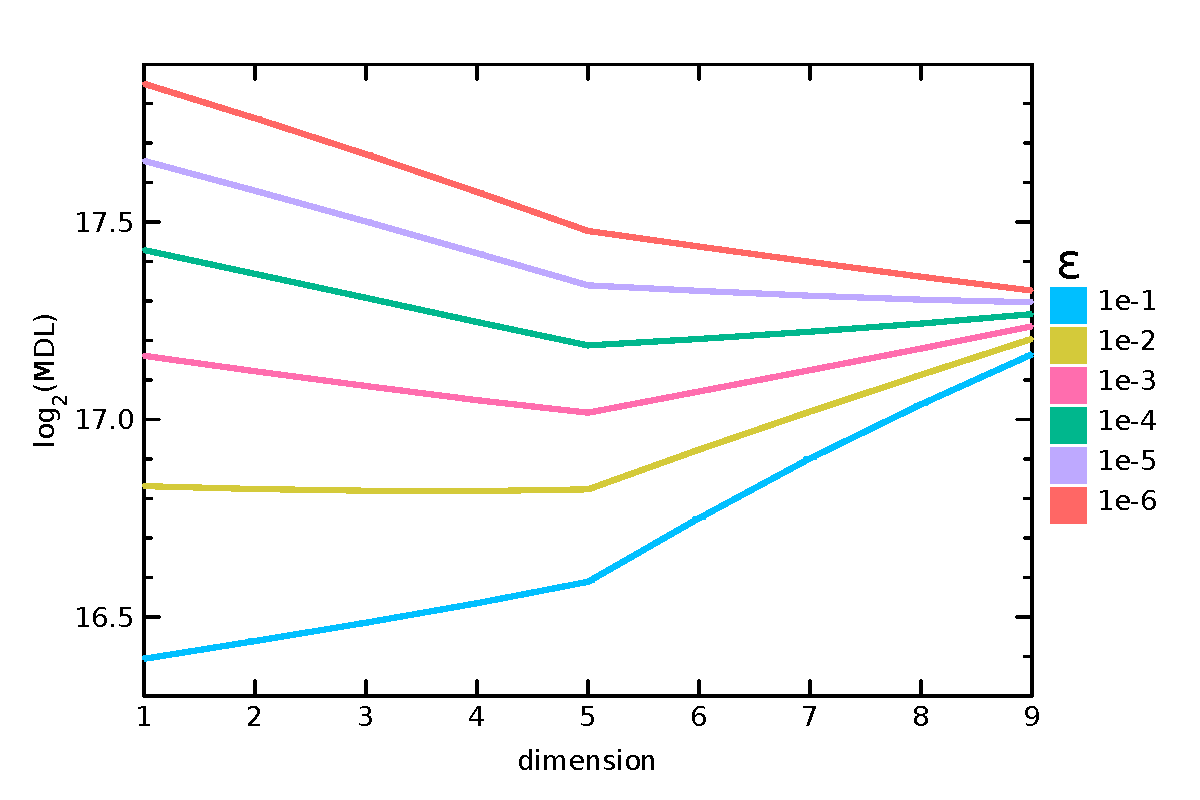
\includegraphics[width=\IfClass{IEEEtran}{3.5in}{4in}]{img/results_mdl-exp5_1.pdf}
\caption{MDL values, calculated with various cluster dimensionality parameters and quantization error \textepsilon for a cluster that is actually a 5D LM cluster in a 10D space.}
\label{fig:mdl-exp5}
\end{figure}



Fig.~\ref{fig:mdl-exp5} shows that MDL value calculated with correct structural
parameters of the examined linear manifold cluster has minimum value when
the dimension parameter corresponds to the cluster dimensionality.
As we established before, see Fig.~\ref{fig:mdl-exp1}, low values of
the quantization error $\varepsilon$ will result in the high cluster MDL value.
High values of $\varepsilon$  will result in the low cluster MDL value.
If the quantization error $\varepsilon$ set to small value, the cluster MDL
value will decreases monotonically with the dimension of cluster.
If the quantization error $\varepsilon$ set to large value, the cluster MDL
value will increases monotonically with the dimension of cluster.
If the quantization error $\varepsilon$ set correctly, the cluster MDL
value will decreases until the right number of dimensions is selected after
which MDL value increases with increasing number of dimension parameter.

% However, when the cluster dimension considered to be lower then the actual one,
% some of the constrained dimensions forced to be quantized. This leads to
% the smaller entropy value in comparison to the proper encoding of the cluster
% when the quantization error is high, or to large values when the quantization
% error is low.
% Similar situation arise when the cluster dimension considered to be higher then
% the actual one, so some unconstrained dimensions are forced to constant encoding
% rather then quantization which results in the larger MDL value in comparison to
% the proper encoding.
      % Results
\subsection{MDL of a Zero-Dimensional Manifold Cluster}
\label{ssc:zero-dim-mdl}




An interesting case arises when we try to calculate the MDL of
a zero-dimensional manifold cluster. Given that a zero-dimensional (ZD)
manifold is a point, any cluster characterized only by its center point is
considered as a zero-dimensional manifold or spherical cluster
\IfClass{IEEEtran}{}{, see Fig.~\ref{fig:zdc}}.
Many clustering algorithms, e.g. $k$-means, produce zero-dimensional manifold
clusters \cite{Jain:1999mf}.

\ifIEEEtran
\else
\begin{figure}[ht]
\center
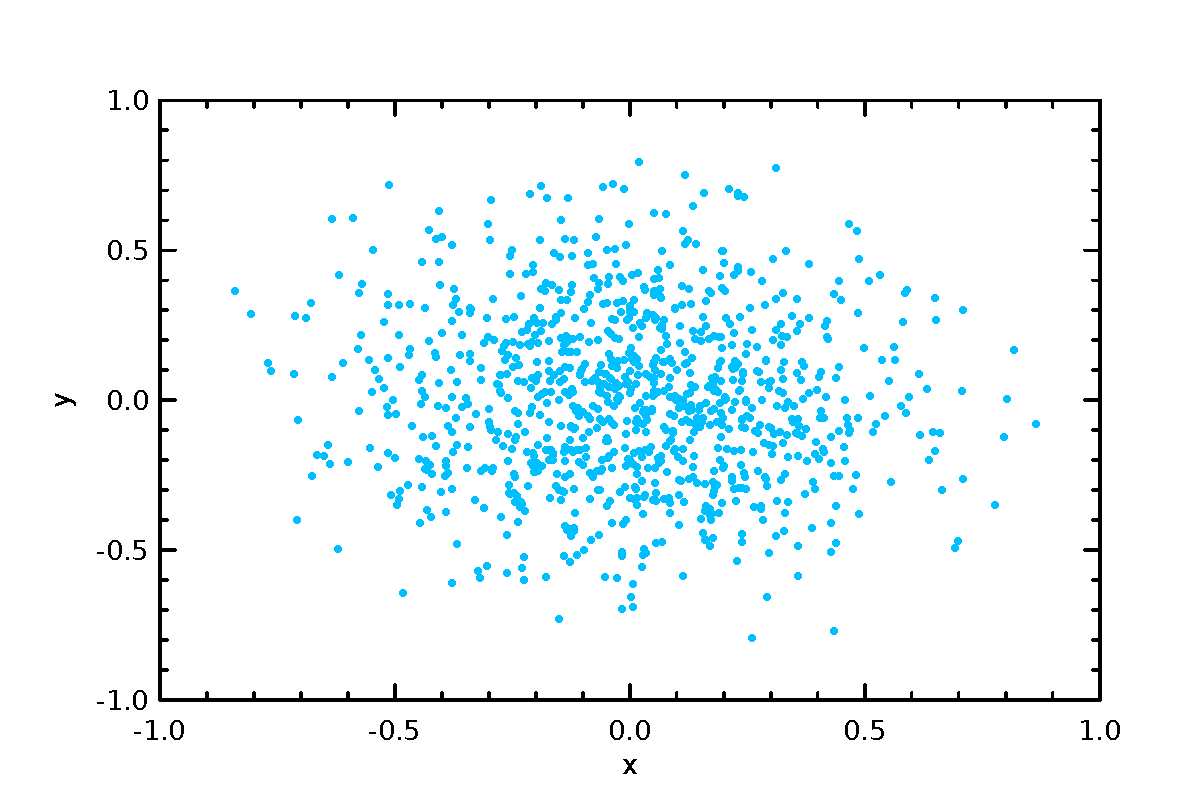
\includegraphics[width=3.5in]{img/zero-dim-mdl_zdc_1.pdf}
\caption{Spherical (zero-dimensional linear manifold) cluster in 2D space}
\label{fig:zdc}
\end{figure}


\fi

Any zero-dimensional manifold cluster is a special case of the linear manifold
cluster, thus we can use encoding (\ref{eq:mdl-lmc-final}) to calculate the MDL
value of the cluster given that dimension of the manifold is zero, $M = 0$.
Thus, (\ref{eq:mdl-lmc-final}) is simplified as follows
\begin{equation} \label{eq:mdl-zdm}
L(\varepsilon) = P_m N + J S(\varepsilon)
\end{equation}

Georgieva et al. \cite{Georgieva:2011tk} took a similar approach in
describing the MDL of zero-dimensional clusters, produced by the $k$-means
algorithm. However, instead of using the entropy of the quantized distribution
of the point positions in particular dimensions, the projection distances to
the point were encoded in MDL as follows
\begin{equation} \label{eq:mdl-zdc}
L = L(H) + L(D|H) = P N + \sum_{i=1}^{J} \sum_{p=1}^{N} \log (d_i^p + 1)
\end{equation}
where $d_i^p$ corresponds to the projection of the distance $d_i$ of
the $i$-th point to the $p$-th dimension.
Such a description does not provide an informative encoding of coordinates when
distances to the center in the cluster are near zero. In such a case, distance
is encoded with less than one bit on the average.

We will compare the degenerate case of the inexact encoding of zero-dimensional
manifold cluster calculated by (\ref{eq:mdl-zdm}) on synthetically generated
linear manifold and spherical clusters. Such an approach will provide a common
ground for comparison between linear manifold and spherical clusters.
We also compare the MDL value of a linear manifold clustering with a cumulative
MDL of a clustering constructed from zero-dimensional clusters which is a more
natural representation of linearly shaped data from the perspective of spherical
clustering algorithms.

% Use 1D manifold (as above) for 0D MDL calculation under various quantization errors.
We used a synthetically generated dataset which has a form of a 1D linear manifold
cluster, an elongated dataset along the one axis, in 2D full space.
Cluster generation procedure was described above.
%described in the section \ref{sc:results}.
We performed the MDL value calculation for the 1D manifold following MDL formula
\eqref{eq:mdl-lmc-final} and then the 0D manifold case defined by \eqref{eq:mdl-zdm}
for various quantization errors.

\begin{figure}[ht]
\center
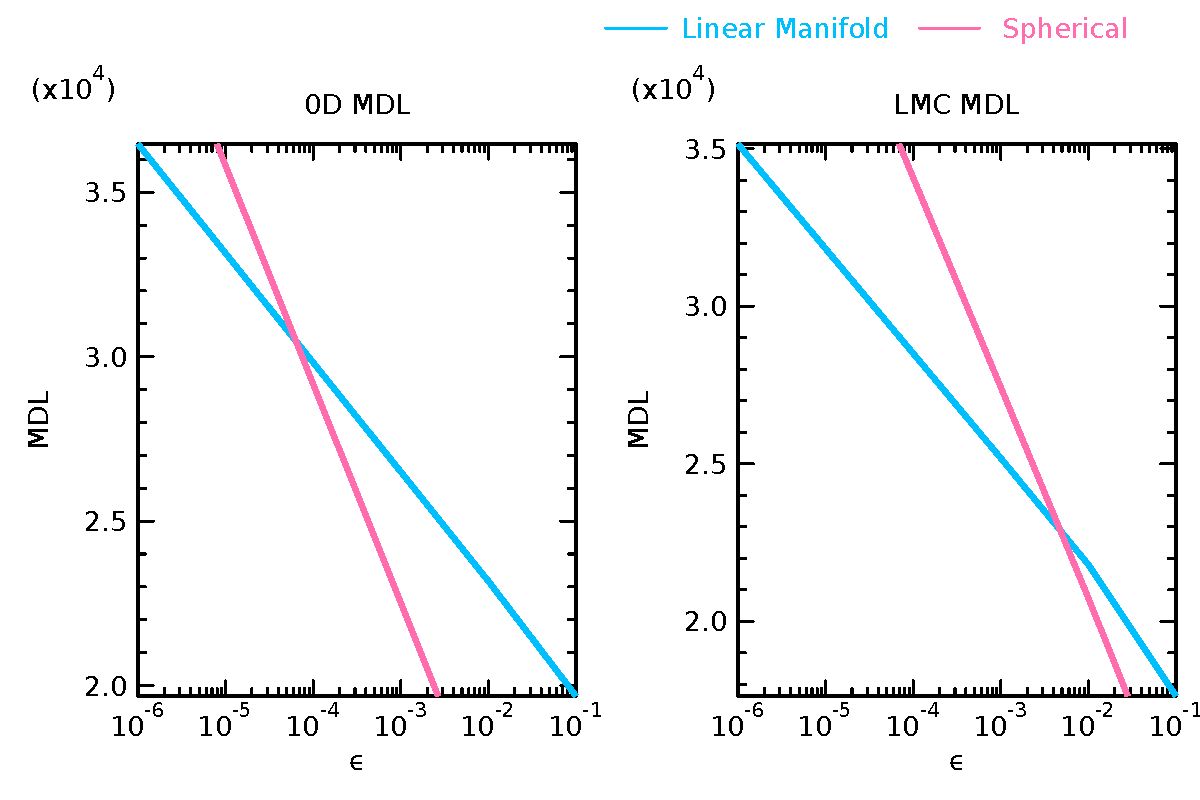
\includegraphics[width=3.5in]{img/zero-dim-mdl_zdc-mdl-exp1_1.pdf}
\caption{Linear manifold (1D) and zero-dimensional (0D) MDL calculations for 1D linear manifold and spherical 0D clusters, located in 2D space, with various quantization errors \textepsilon.}
\label{fig:zdc-mdl-exp1}
\end{figure}



Figure~\ref{fig:zdc-mdl-exp1} shows results of linear manifold Eq.~\eqref{eq:mdl-lmc-final}
and zero-dimensional Eq.~\eqref{eq:mdl-zdm} MDL value calculations for various types
of manifold clusters. For large quantization errors, both approaches to the MDL
calculation produce a small MDL value for spherical cluster. However, when
the precision of the quantization procedure increases, resulting in a more
complete and informative description of the cluster, the MDL value of the linear
manifold cluster becomes smaller than the spherical cluster regardless of
the selected method of calculation.
% Although, LM-MDL approach provides smaller value of the linear
% manifold cluster under the larger quantization error, then ZD-MDL approach.
\IfClass{IEEEtran}{}{\bigskip}

%Use k-means to cluster 1D linear manifold, k>=1, and calculate total MDL of clustering. Compare resulted value to the MDL of 1D LM.

Because of the structural difference between linear manifold and spherical
clusters, it is hard to come with common criteria for comparison of
different types of clusters. We use the MDL value as a measure for
heterogeneous cluster comparison. In order to test how the cluster MDL would
perform as a comparison score, we calculated MDL values of synthetically
generated clusters of different types - linear manifold and spherical.

We generated a 1D linear manifold cluster dataset from a bivariate normal
distribution, as in previous experiments, and used the $k$-means algorithm to
synthesize spherical clusters from it. We varied the number of clusters for
the $k$-means algorithm that allowed us to form clusters which gradually
obtain a spherical shape, as the linear manifold cluster got partitioned
into more clusters.

We perform an evaluation of the MDL value for the linear manifold clusters by
Eq.~\eqref{eq:mdl-lmc-final} and spherical cluster by Eq.~\eqref{eq:mdl-zdm}.
When $k$-means generated more than one cluster from the original dataset,
we summed all the cluster MDL values in the clustering to obtain
the MDL score for the original 1D LM cluster represented by the dataset.
\IfClass{IEEEtran}{This is shown in Figure~\ref{fig:mdl-zdc-exp2}.}{}

\begin{figure}[ht]
\center
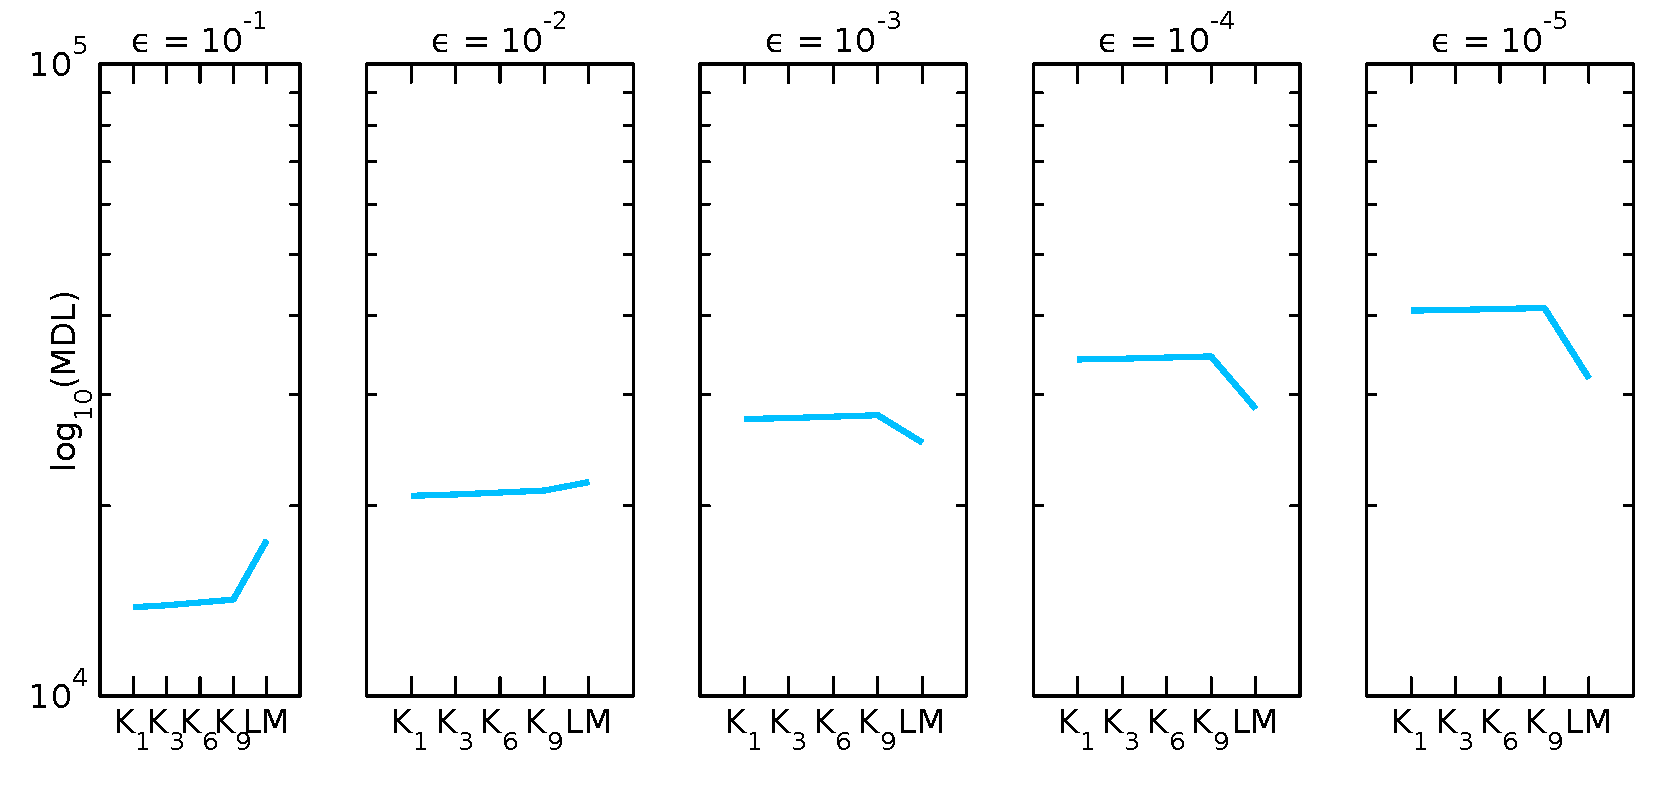
\includegraphics[width=3.5in]{img/zero-dim-mdl_zdc-mdl-exp2_1.pdf}
\caption{MDL value of k-means clusterings (K[k]) produced from the 1D linear manifold cluster (LM), located in 2D space, under various quantization errors \textepsilon.}
\label{fig:zdc-mdl-exp2}
\end{figure}



\IfClass{IEEEtran}{}{
Figure \ref{fig:mdl-zdc-exp2} shows results of MDL calculations for clusterings
produced from the 1D linear manifold cluster.}We found that the division of
the linear manifold on multiple spherical clusters does not provide much
difference in the resulted MDL value. As in the previous experiment, the major
factor which affects MDL calculations is the quantization error parameter.
For a small quantization error, spherical clusters provide a smaller MDL value
for the experimental dataset. Moreover, the MDL value of the whole dataset does not
increase significantly with the number of clusters in the $k$-means clustering.
However, as the quantization error decreases, the MDL value calculated by
Eq.~\eqref{eq:mdl-lmc-final} becomes significantly smaller then the spherical
cluster MDL value Eq.~\eqref{eq:mdl-zdm}.

This result suggests that for a large quantization error a spherical description
of the linear manifold cluster provides more compact MDL value over
the linear manifold MDL model. But while the quantization error decreases,
giving a better description of the data, the linear manifold MDL model produces
more compact encoding of the linear manifold cluster and outperforms the spherical
MDL model regardless of cluster proximity to true spherical representation.
 % MDL of zero-dimensional manifold
\subsection{Using MDL Heuristic in Climate Data Clustering}
\label{ssc:climate}

We added the linear manifold clustering MDL heuristic into the LMCLUS algorithm,
and tested clustering performance on climate datasets.

Our dataset comprised of subset of the CRU 3.22 dataset of monthly global
surface temperature averages, and Global Precipitation Climatology Centre
(GPCC) dataset of monthly precipitation averages, for a 30 year period form
1951 to 1980.
Original datasets have the same $1^\circ \times 1^\circ$ resolution.
Both datasets are 12 dimensional, so the combined dataset has 24 dimensions.
For each of group of 12 fields, a unit length normalization was performed,
by subtracting the minimum value from every point and divided it by the field
maximum minus the minimum value. Normalization makes the scale of the disparate
temperature and precipitation fields similar.

The K{\"o}ppen-Geiger (KG) climate classification system is a widely used scheme
developed by geographers to classify climate types correlated  with observed
land ecosystems \cite{Koppen:1936dg}. It is based on observed limits of these
ecosystems relative to seasonal or annual precipitation and temperature.
A recent updated version identifies 34 climate classes \cite{Kottek:2006wd}.
The system is not perfect, so variations are often proposed.  However, on
the hypothesis that ecosystem types are an expression of the climate,
the KG system offers a good benchmark for a clustering analysis.
\IfClass{IEEEtran}{}
{
Because the KG system relies on at least seasonal (4) and annual values for
temperature and precipitation, it may be considered 10-dimensional clustering or
classification. Thus, we expect $k$-means clustering to yield less accurate
classes, and  linear manifold clustering might identify more refined classes.
(It is beyond the scope of this paper whether LMC offers improved climate
classification over that derived by geographers' expert knowledge, but this will
be treated in a later paper).
}

We perform clustering of the above climate dataset using following algorithms:
$k$-Means \cite{Jain:1999mf}, ORCLUS \cite{Aggarwal:2000AY}, original
LMCLUS \cite{Haralick:2007rt} and LMCLUS modified with the MDL heuristic.

The $k$-Means clustering assumes that the data is modeled as a mixture of
spherically shaped distributions. In this model, the cluster ideal is a point,
the cluster center, which is its mean, and the observations are isotropically
perturbed around the mean. Because the number of clusters must be set a priori
for $k$-Means, with the climate data clustering, we set this number to 34 to
match the number of Koeppen-Geiger classes. Similarly to $k$-Means, ORCLUS
requires an exact number of clusters as a parameter, but the resulting clusters
are linear manifolds of the dimension specified by one of the parameters.
We set ORLCUS parameters such that the algorithm would generate 34 1D linear
manifold clusters.

Linear Manifold Clustering (LMCLUS) does not have to specify an exact number of
clusters in advance, but there are multiple parameters that affect performance
of the algorithm. We set only a small group of them, the rest of the parameters
were set to their default values. The effect of the parameters
\IfClass{IEEEtran}{}{
\footnote{Appendix section~\ref{sec:lmclus-params} contains LMCLUS parameters,
their description and default values.}
}
on the clustering performance is described in the original paper \cite{Haralick:2007rt}.
In our experiments, the following LMCLUS parameters were set:
\emph{best\_bound} to 0.4, \emph{sampling\_factor} to 0.1,
\emph{number\_of\_clusters} to 34, \emph{min\_cluster\_size} to 150.

We updated LMCLUS with the MDL heuristic that allowed a goodness evaluation
of the prospective manifold cluster before committing to the partitioning of
this clusters from the rest of the dataset. We calculated a compression ratio
as a ratio between ``raw'' cluster encoding, as a total number of bits required
to encode each point of the cluster with a constant precision, and
the cluster MDL encoding. If the compression ratio is larger than a user
specified threshold, the cluster is accepted.

In order to compare the goodness of produced clusterings, we calculated
the total MDL value of the resulting clustering for each algorithm as a sum of
cluster MDL values. We performed the total MDL calculation with various
quantization error values to understand how precision affects it.

We calculated value of the approximate MDL Eq.~\eqref{eq:mdl-lmc-final} for
the climate data clusterings, generated by various algorithms, with
the quantization error $\varepsilon$ in
the interval $\left[0.001, 0.002, \dots, 0.01 \right]$.
Because the quantization error is a parameter for the MDL heuristic,
we calculated separate clusterings for every $\varepsilon$ value in
the specified interval. Moreover, the quantization error affects the calculation
of the compression ratio, thus the compression ratio parameter was
selected different for every clustering calculation as well.
We used the clustering, generated by the original LMCLUS algorithm, for
calculation of an average $\mu$ and a standard deviation $\sigma$ of
a cluster compression ratio at every $\varepsilon$ value.
These statistics were used to bootstrap the compression ratio parameter
for the MDL heuristic. The compression ratio set to $\mu-\sigma/2$ value for
corresponding $\varepsilon$ value.

Figure~\ref{fig:mdl-error} shows that when MDL heuristics is enabled, it
produced clusterings that are slightly different from the clustering generated
by original method. We suspected that Eq.~\eqref{eq:mdl-lmc-final} does not
appropriately reflect the MDL value of the the distribution of the data points
in each of the clusters.

\begin{figure}[ht]
\centering
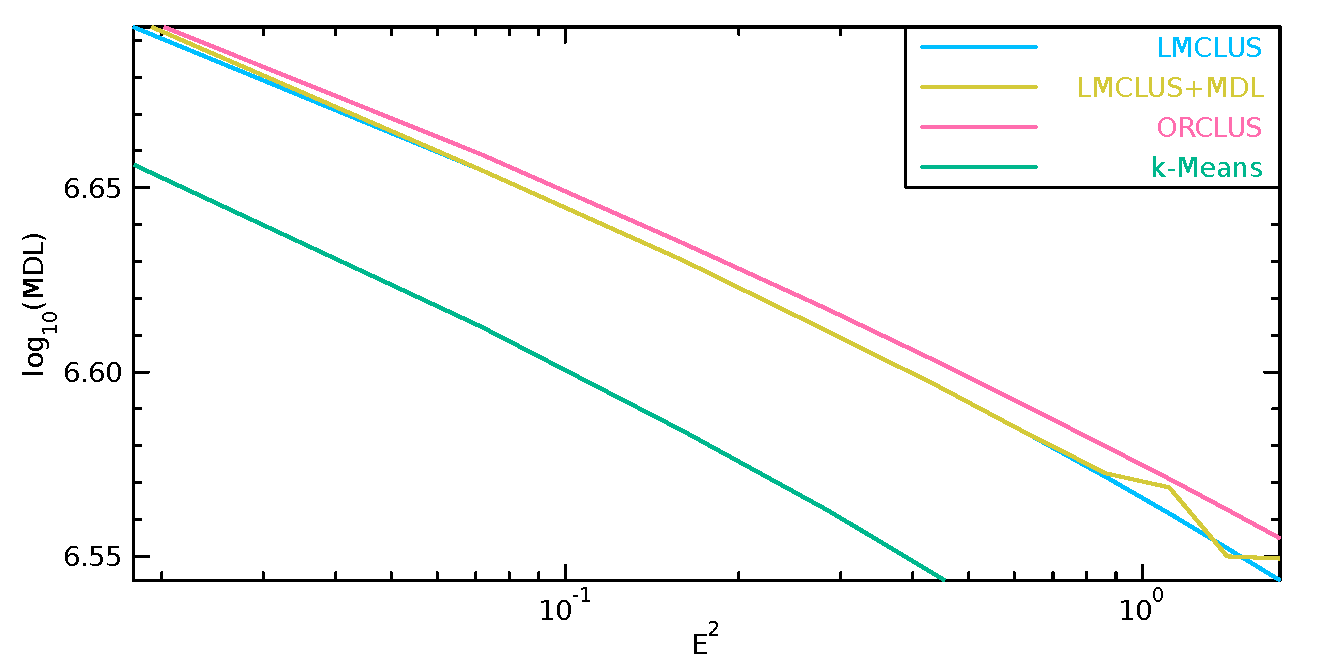
\includegraphics[scale=\IfClass{IEEEtran}{0.3}{0.5}]{img/toterrs2-mdl-oq.pdf}
\IfClass{IEEEtran}{\vspace*{-10pt}}{}
\caption{Clustering optimal quantization MDL value \eqref{eq:mdl-lmc-final} and its squared quantization error for $\varepsilon$ in interval $\left[0.001, 0.002, \dots, 0.01 \right]$ and various algorithms.}
\label{fig:mdl-error}
\end{figure}

When we switched to the ``population'' MDL Eq.~\eqref{eq:mdl-lmc-final-pop}
calculations in our MDL heuristics, with the parameters accordingly recalculated
for this algorithm, performance of the clustering algorithm considerably improved.

It became clear that the effect of the MDL heuristics of resulting clustering,
see Figure~\ref{fig:mdl-error-pop}, are aligned with results from the synthetic
simulation from section \ref{ssc:zero-dim-mdl}. Increasing the precision of
the linear manifold MDL calculation results in better goodness-of-fit qualities
of clusters and allows the filtering of subpar cluster candidates during
the LMCLUS stochastic search, which improves the final clustering.

\begin{figure}[ht]
\centering
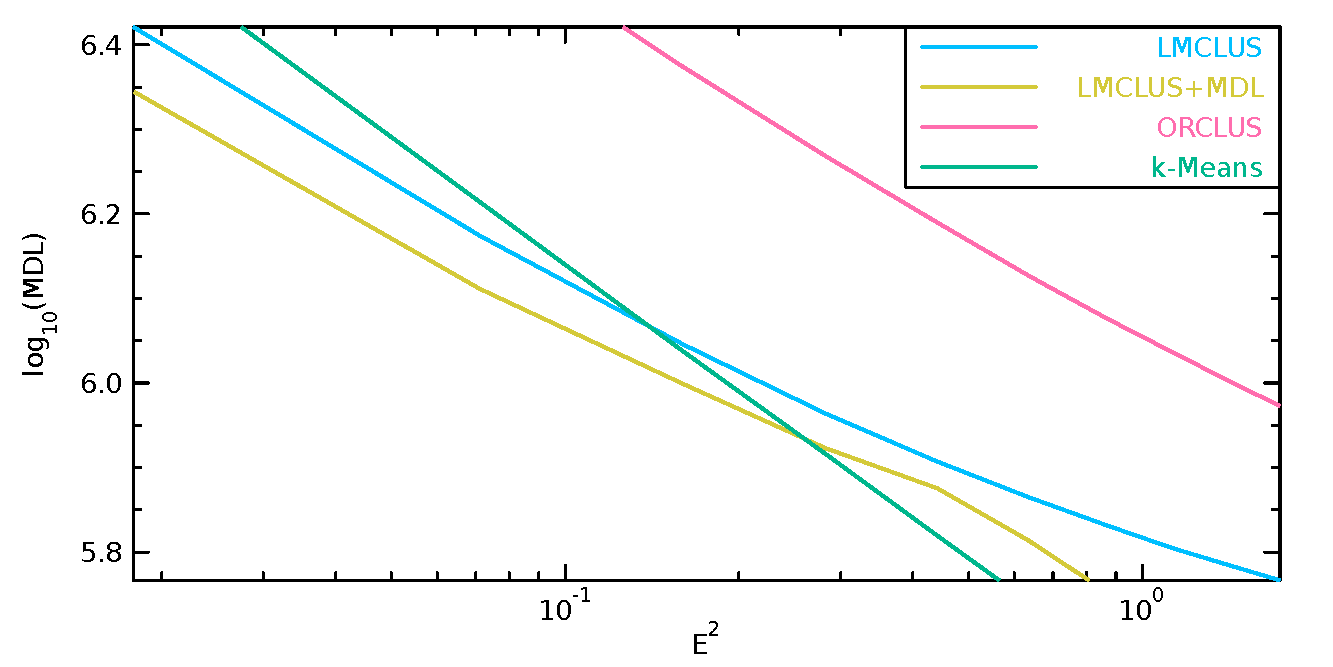
\includegraphics[scale=\IfClass{IEEEtran}{0.3}{0.5}]{img/toterrs2-mdl-si.pdf}
\IfClass{IEEEtran}{\vspace*{-10pt}}{}
\caption{Clustering population MDL value \eqref{eq:mdl-lmc-final-pop} and its squared quantization error for $\varepsilon$ in interval $\left[0.001, 0.002, \dots, 0.01 \right]$ and various algorithms.}
\label{fig:mdl-error-pop}
\end{figure}


\IfClass{IEEEtran}{}{
Figure~\ref{fig:cl-climate} show resulted clusterings plotted on the world map,
where patches of the land are associated with particular clusters.
%
\begin{figure}[ht]
\captionsetup{justification=centering,margin={0cm,-2cm}}
\vspace*{-20pt}
\hspace*{-15pt}
\subfigure[LMCLUS]{
    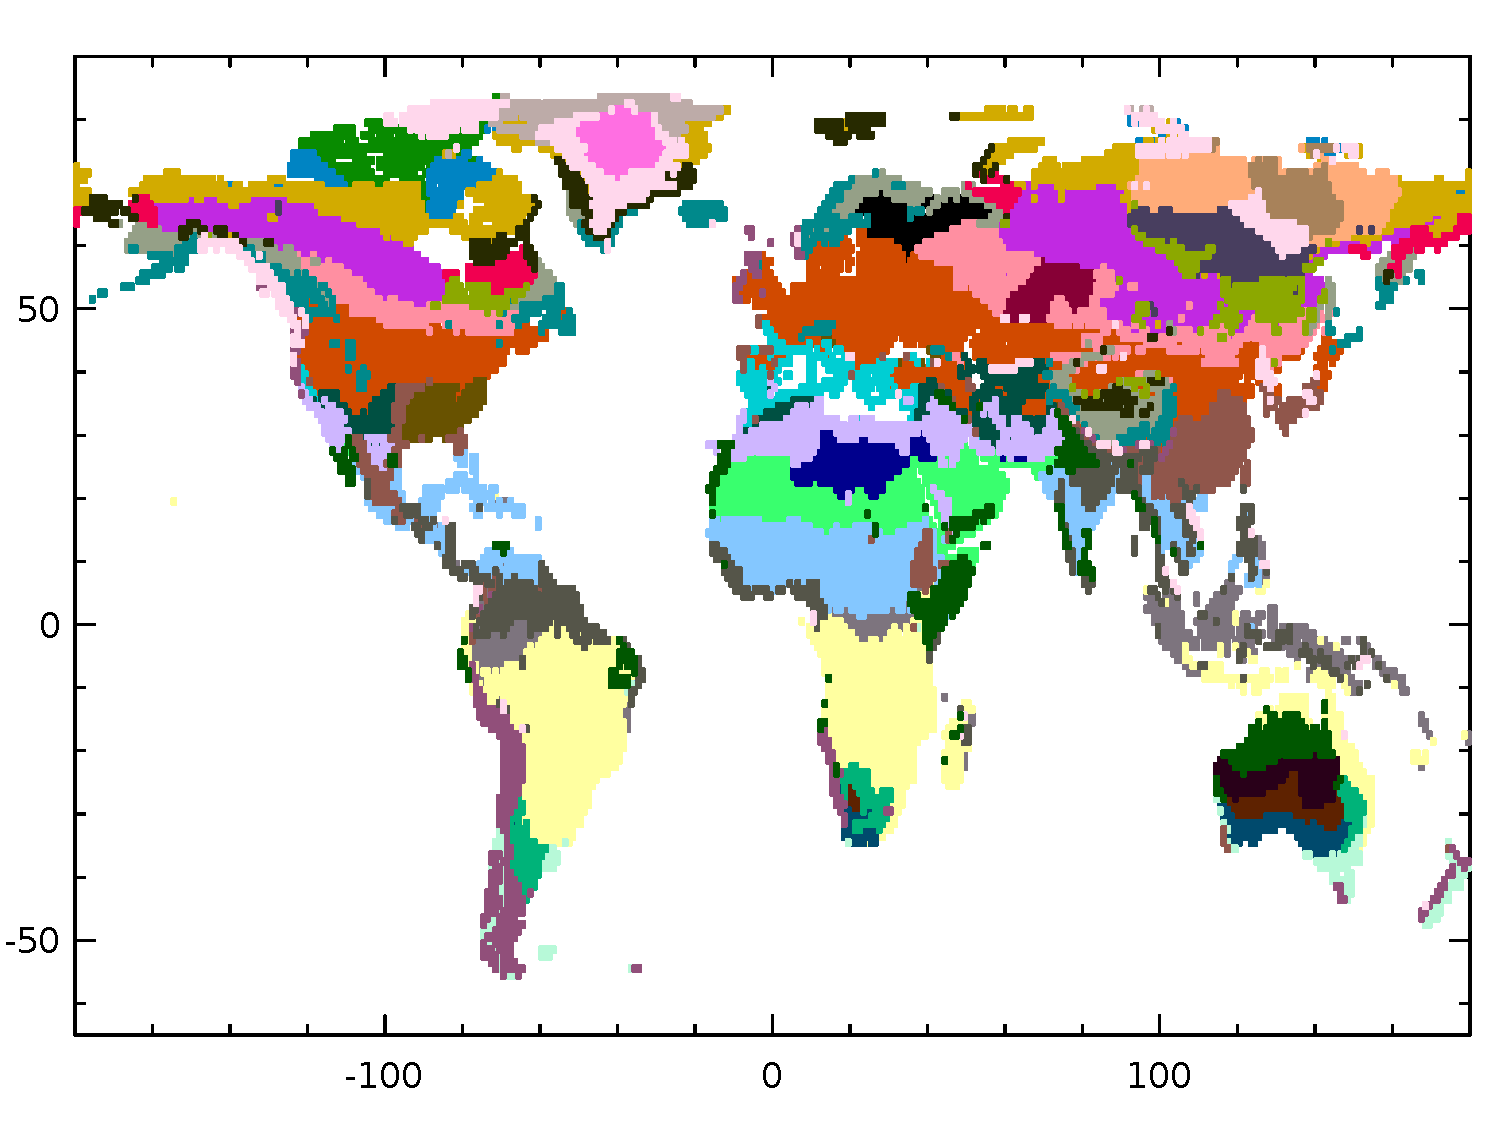
\includegraphics[width=3.5in, height=2.5in]{img/icpr-cl-lmclus.pdf}
    \label{fig:cl-lmclus}}
\hspace*{-15pt}
\subfigure[LMCLUS-MDL]{
    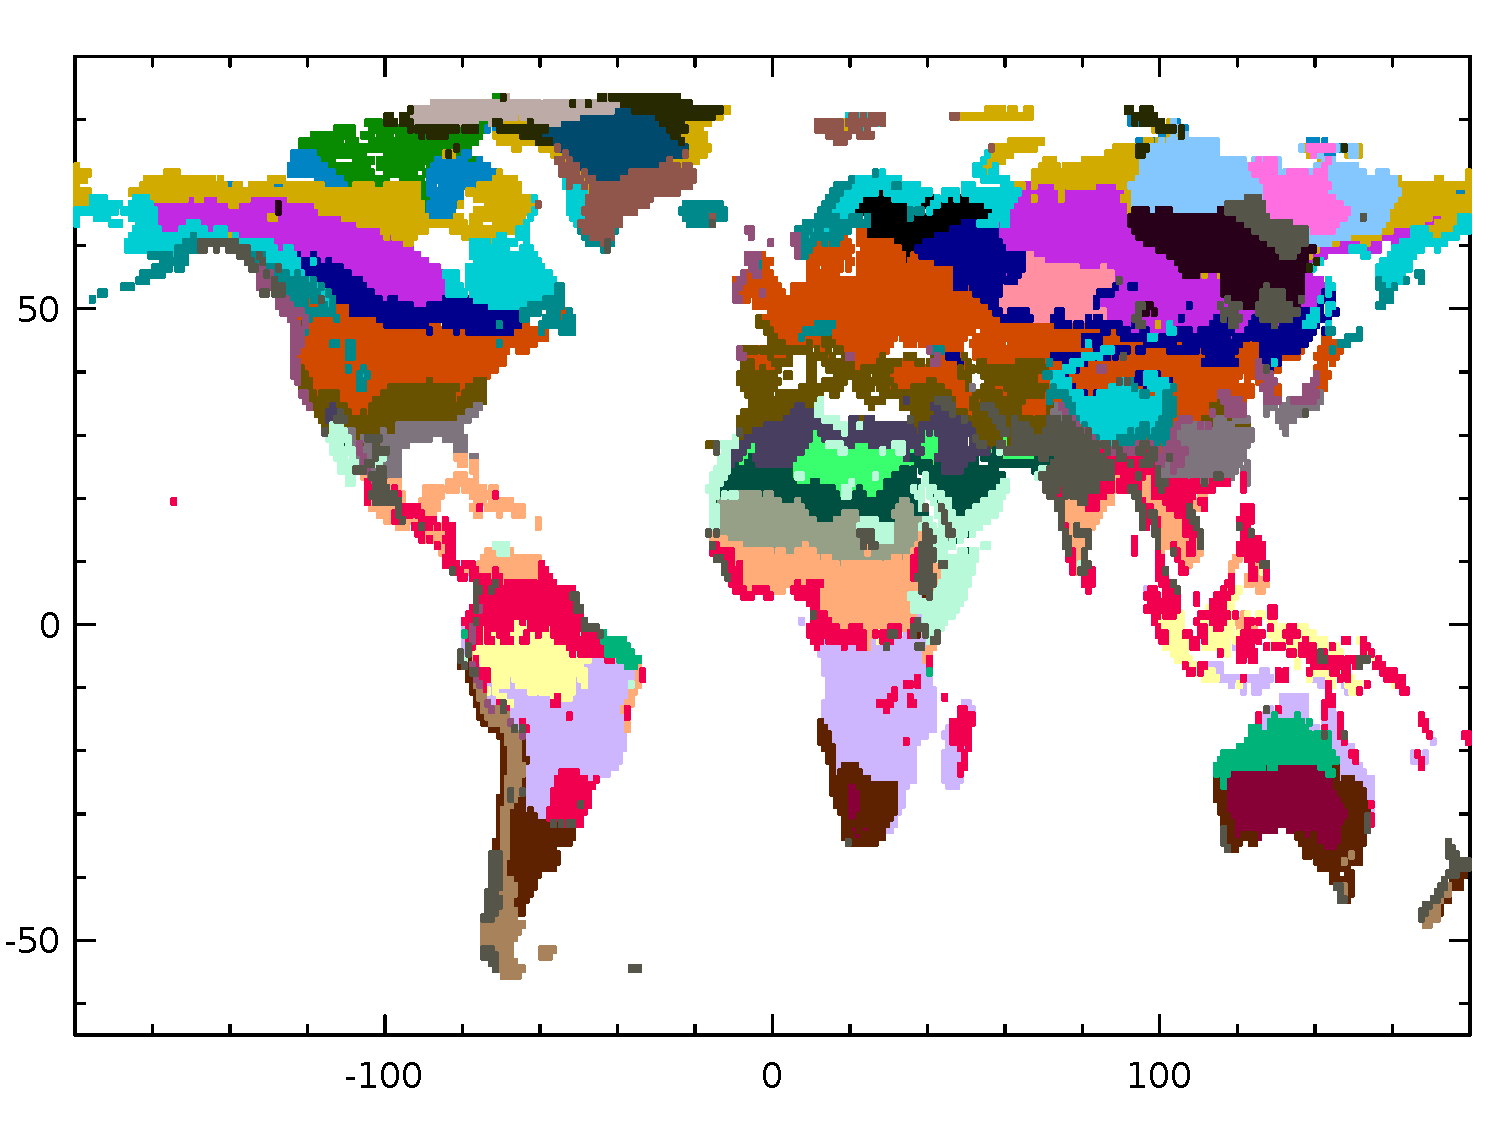
\includegraphics[width=3.5in, height=2.5in]{img/icpr-cl-lmcmdl.pdf}
    \label{fig:cl-lmcmdl}}
\hspace*{-15pt}
\subfigure[$k$-Means]{
    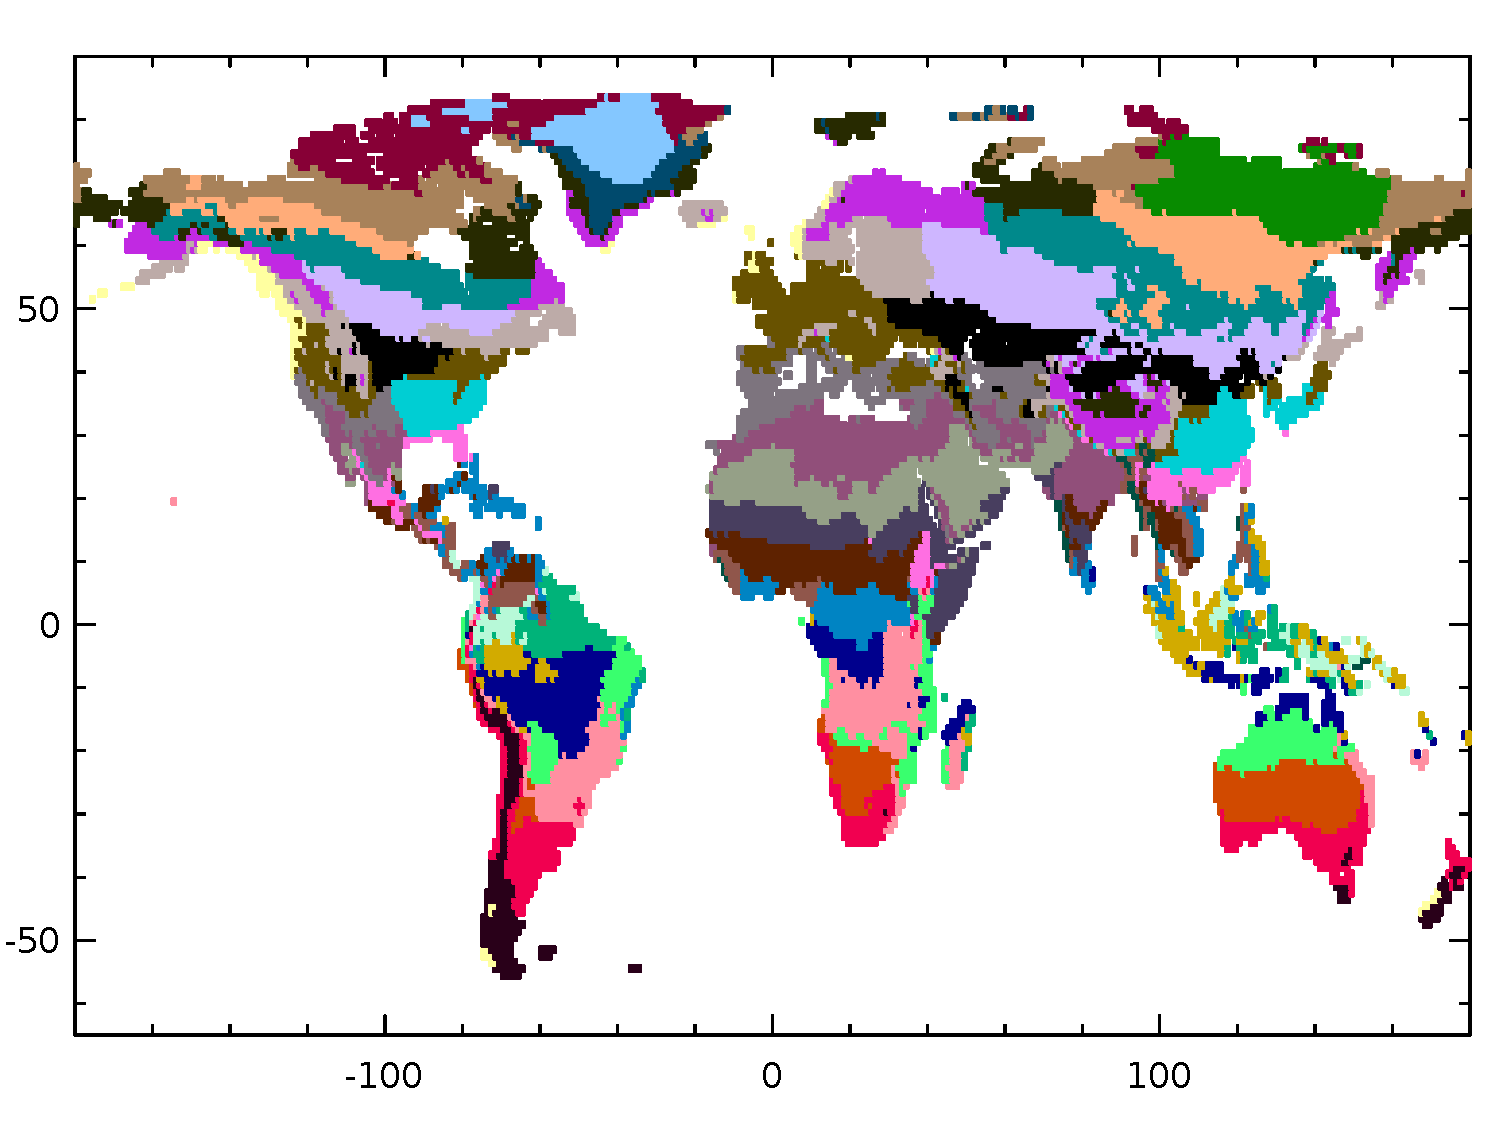
\includegraphics[width=3.5in, height=2.5in]{img/icpr-cl-kmeans.pdf}
    \label{fig:cl-kmeans}}
\hspace*{-15pt}
\subfigure[ORCLUS]{
    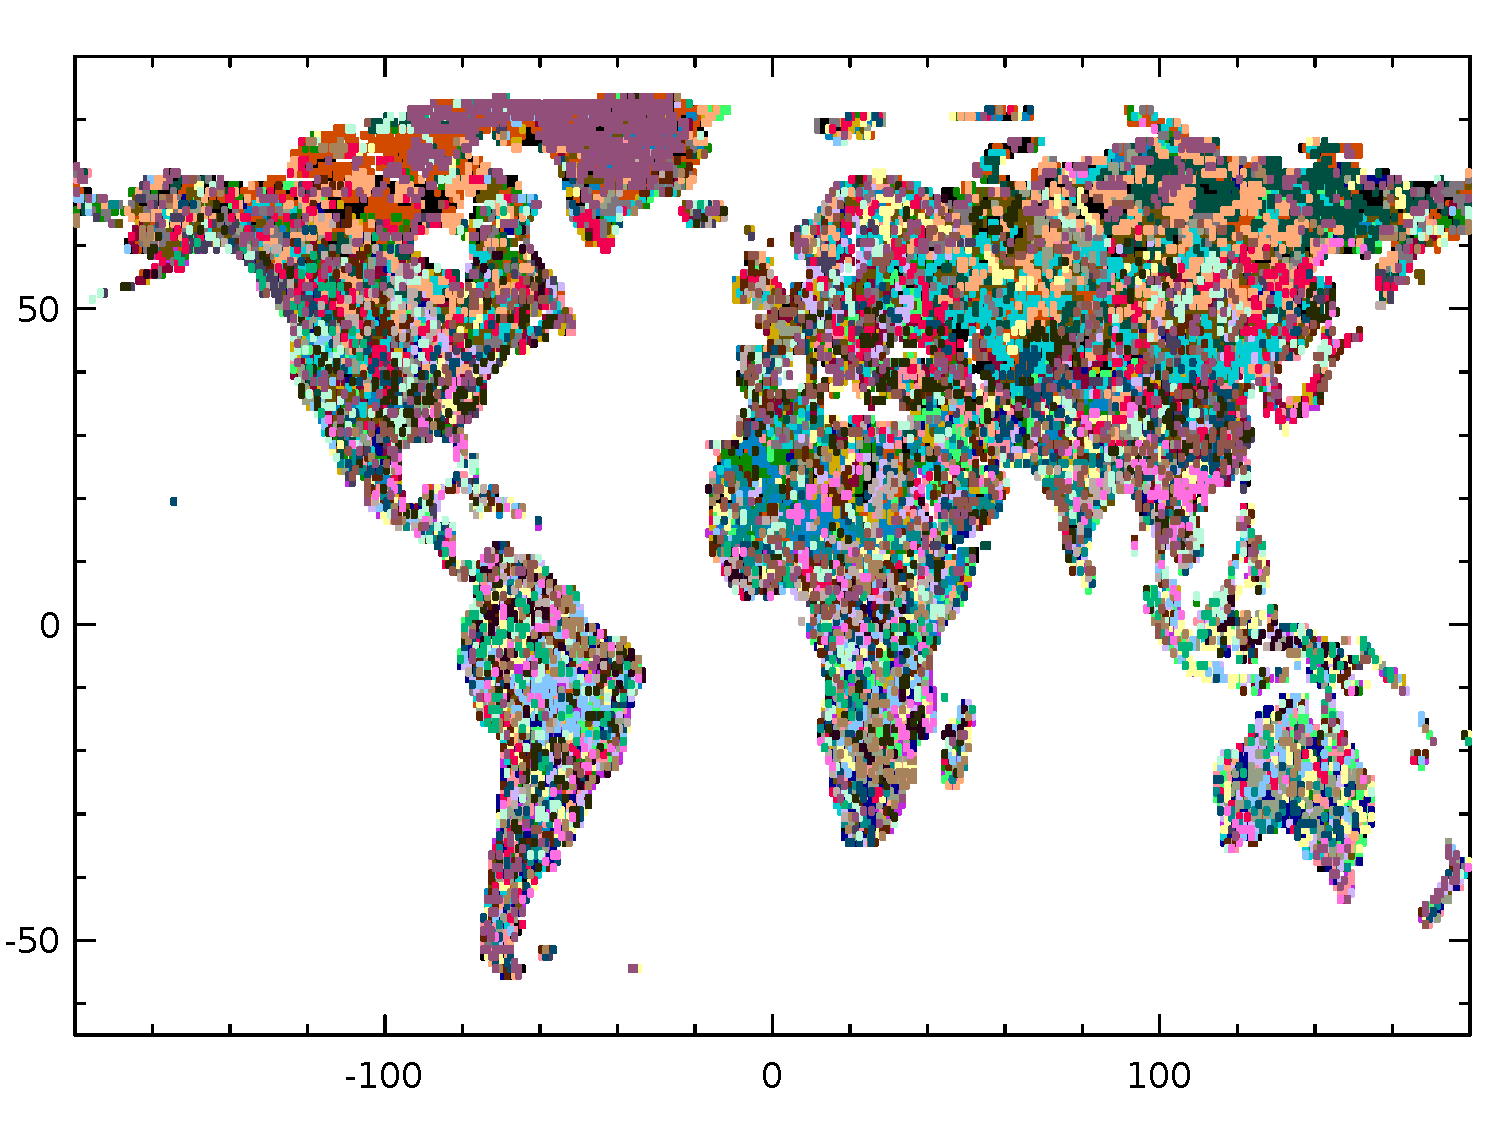
\includegraphics[width=3.5in, height=2.5in]{img/icpr-cl-orclus.pdf}
    \label{fig:cl-orclus}}
% \hspace*{-15pt}
\hspace*{0.25\textwidth}
\subfigure[K{\"o}ppen-Geiger]{
    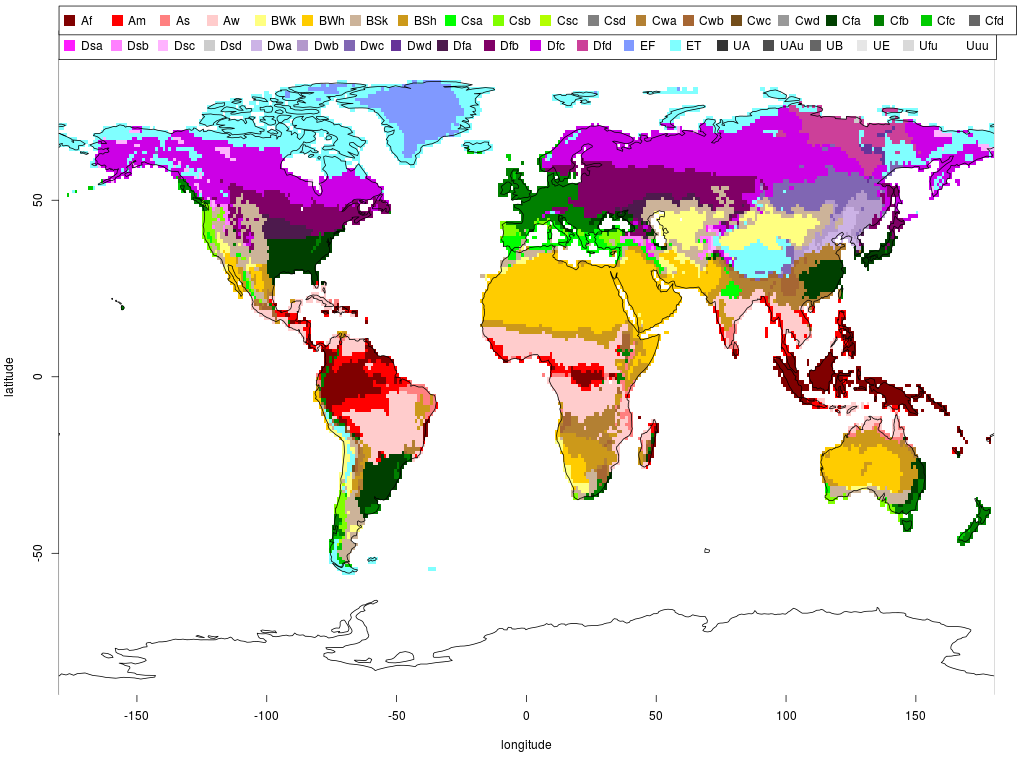
\includegraphics[width=3.5in, height=2.5in]{img/CL-KG.png}
    \label{fig:cl-kg}}
\caption{
    Results of clustering of the 24D climate dataset, composed of monthly
    averages of temperature (CRU) and precipitation (GPCC) during 1951-1980
    period, by LMCLUS \subref{fig:cl-lmclus}, by LMCLUS+MDL \subref{fig:cl-lmcmdl},
    by ORCLUS \subref{fig:cl-orclus} and $k$-Means \subref{fig:cl-kmeans}
    algorithms. For reference, K{\"o}ppen-Geiger classification is given in \subref{fig:cl-kg}.
    \emph{Note: Colors represents associations of grid cells to particular
    clusters. There is no correspondence between colors on displayed plots.}
}
\label{fig:cl-climate}
\end{figure}
}

% \IfClass{IEEEtran}{}{
% In order to compare goodness of produced clusterings we calculated the total MDL
% value of the resulting clustering for each algorithm as a sum of cluster MDL
% values. We performed the total MDL calculation with various quantization error
% values to understand how precision affects the goodness criteria.
% Figure~\ref{fig:cl-mdl} shows the effect of quantization error on the MDL value
% of clustering.
% It is clear that linear manifold clusters, which have an intrinsic
% linear structure, show better goodness-of-fit qualities reflected in
% the smaller total MDL value than the spherical zero-dimensional clusters
% produced by $k$-Means algorithm.
% %
% \begin{figure}[ht]
% \IfClass{IEEEtran}{\vspace*{-10pt}}{}
% \centering
% \includegraphics[width=3.5in]{img/cl-mdl.pdf}
% \IfClass{IEEEtran}{\vspace*{-35pt}}{}
% \caption{Total MDL value for climate dataset clustering, produced by LMCLUS and $k$-Means algorithms calculated for various user-set quantization error values.}
% \label{fig:cl-mdl}
% \end{figure}
% }
      % Results of climate clustering
\ifIEEEtran
\else
\subsection{MDL Precision Error}
\label{ssc:mdl-error}

% In our experiments with linear manifold clusters, we use following definition of
% the minimum description length,
% \begin{equation} \label{eq:mdl-lmc-final}
% L(\varepsilon)
%     % = P_m [N + M(N - (M+1))/2 ]+ n(P_d\cdot M  + S(\varepsilon))
%     = P \sum^K_{k=1} \left[ N \cdot (N+3)/2 + 2 \sum^N_{m=M_k} Q_{mk}(\varepsilon) \right]
% \end{equation}
% where
% \begin{itemize}
% \item $N$ is the dimension of the space,
% \item $M$ is the dimension of the manifold,
% \item $n$ is a number of points in the linear manifold cluster,
% \item $P_m$ is the number of bits used for encoding each component of
% the manifold translation and the numbers required to calculate the basis vectors,
% \item $P_d$ is the number of bits used for encoding $M$ components of
% cluster point, projected on the linear manifold,
% \item $S(\varepsilon)$ is an entropy of a distribution of cluster points,
% in the orthogonal compliment subspace to the linear manifold of the cluster,
% calculated to be correct within an error bound of  $\varepsilon$,
% \item $\varepsilon$ is the specified quantization error.
% \end{itemize}

We are going to investigate the precision of the MDL calculations, in particular,
how changes in the encoding of the model and data affects resulting MDL value.

% Setup



For our experiments we used results of the climate clustering dataset,
see Section \ref{ssc:climate}. The climate dataset is the 24D dataset composed
of temperature and precipitation monthly averages for the period form 1951-1980.
We used cluster number 2, see Fig.~\ref{fig:cl-lmclus-c2}, which is a one
dimensional cluster, from the above clustering results.

\begin{figure}[H]
\centering
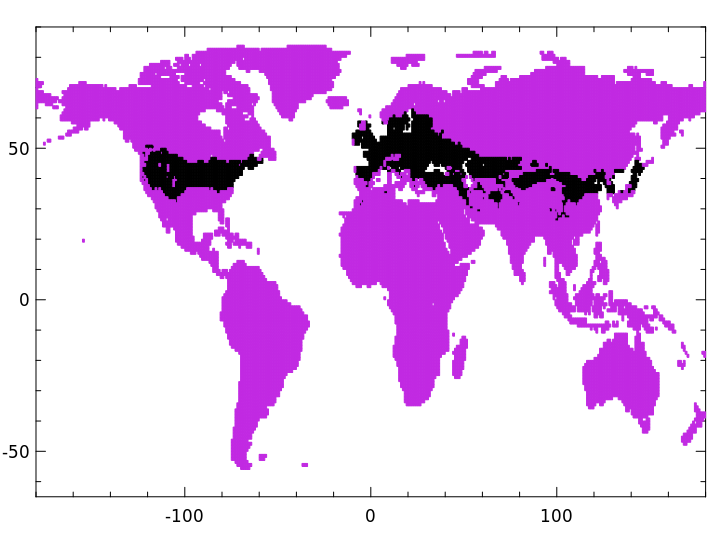
\includegraphics[width=3.5in]{img/CL02.png}
\caption{Cluster \#2 of the climate dataset created by LMCLUS algorithm, see Figure \ref{fig:cl-lmclus} in Section \ref{ssc:climate}.}
\label{fig:cl-lmclus-c2}
\end{figure}

First, we looked at the error introduced by the encoding of the data with
the lower precision then computations were done with. By default, $P_d$ constant
is set to 16 bits, which corresponds to the half-precision floating-point format,
\emph{Float16}. However, computations are usually done can be done in
the single-precision, \emph{Float32}, or double-precision floating-point format,
\emph{Float64}.

Error is calculated as difference between projected points in different
precision,
\begin{equation}
E_p = \frac{1}{n} \sum^n_{i=1} || B'x_i - q(B'x_i) ||^2
\end{equation}
where $B$ is the basis of the manifold in computational precision,
$x_n$ is the manifold point in computational precision,
$q$ is the conversion function from computational to encoding precision.

% precision error for projected data

\begin{juliaterm}
julia> #
# Encoding of the data from Float32 to Float16
prec_error(B,Xt,Float32,Float16)
1.5530144f-5

julia> 
# Encoding of the data from Float64 to Float16
prec_error(B,Xt,Float64,Float16)
1.5529915950350614e-5

julia> 
# Encoding of the data from Float64 to Float32
prec_error(B,Xt,Float64,Float32)
1.858106839030262e-9

\end{juliaterm}



Next, we verify that the quantization error within the user specified value
$\varepsilon$ for the encoding of the linear manifold cluster points in
the orthogonal compliment space. We calculated the average expected quantization
error $E$ and the average actual quantization error $E_q$.

% quantization error for projected data



\begin{table}[h]
\center
\begin{tabular}{ccc}
$\varepsilon^2$ & $E^2$ & $E_q^2$ \\
\hline
1.000e-04 & 1.005e-04 & 9.307e-03 \\
1.000e-06 & 9.994e-07 & 9.055e-05 \\
1.000e-08 & 1.000e-08 & 9.090e-07 \\
1.000e-10 & 1.000e-10 & 9.066e-09 \\



\end{tabular}
\caption{Average expected, $E$, and actual, $E_q$, quantization errors for
particular user-defined quantization error upper boundary $\varepsilon$.}
\label{tbl:quant-error}
\end{table}

Comparison results, see Table~\ref{tbl:quant-error} show that squared expected
quantization error \eqref{eq:sq-quant-error}, $E^2$, is under the user-defined
error upper boundary, $\varepsilon^2$. However, the actual squared quantization
error, $E_q$, resulted from quantizing the cluster points under calculated
quantization parameters \eqref{eq:quant-intervals}, is much larger then
expected one for a loose error boundary. But this error approaching to
its expected value as quantization error boundary tightens.

\subsection{Clustering Minimal Description Length}
\label{ssc:mdl-clust}

In this section we analyze changes in the LM minimal description length values
when it is computed for a collection of clusters of arbitrary dimension and size
-- clustering.

For our experiments we performed clustering of the climate dataset,
see Section \ref{ssc:climate}. We performed multiple clusterings of the dataset
varying only one parameter -- \emph{best\_bound}. This parameter affect
cluster partitioning mechanism in LMCLUS algorithm which influence a final
number of generated clusters \cite{Haralick:2007rt}. We generate a sample
composed of clusterings produced by changing \emph{best\_bound} parameter in
range [0.1, 1.2] with value increment of 0.05. This results in 23 clusterings
per each clustering sample. For a statistical evaluation, we collected 1000
clustering sample, total 23000 clusterings.

For the reference to the K{\"o}ppen-Geiger (KG) climate classification system that
identifies 34 climate classes, we set \emph{number\_of\_clusters} parameter,
an expected number of clusters for the LMCLUS algorithm, to 34.
This parameter affects sampling procedure for a manifold basis of a prospective
cluster \cite{Haralick:2007rt}.

In our experiments, we also set minimum cluster size parameter,
\emph{min\_cluster\_size}, to 150, and sampling factor parameter,
\emph{sampling\_factor}, which is used in the sampling heuristics to constrain
a number of samples for potential cluster linear manifold, to 1.0.
Rest of the LMCLUS algorithm parameters where set to default values.
For more detailed description of LMCLUS algorithm parameters consult
Table~\ref{tab:lmclus-params} in the Appendix~\ref{ssec:lmclus-params}.

% Setup



\subsubsection{Parameters of Clusterings}
\label{sssc:clust-params}

We analyzed a clustering size, which is a number of clusters in the clustering,
gathered from generated clustering samples. First, we group all clusterings by
their sizes with respect to \emph{best\_bound} parameter.

\begin{figure}[H]
\center
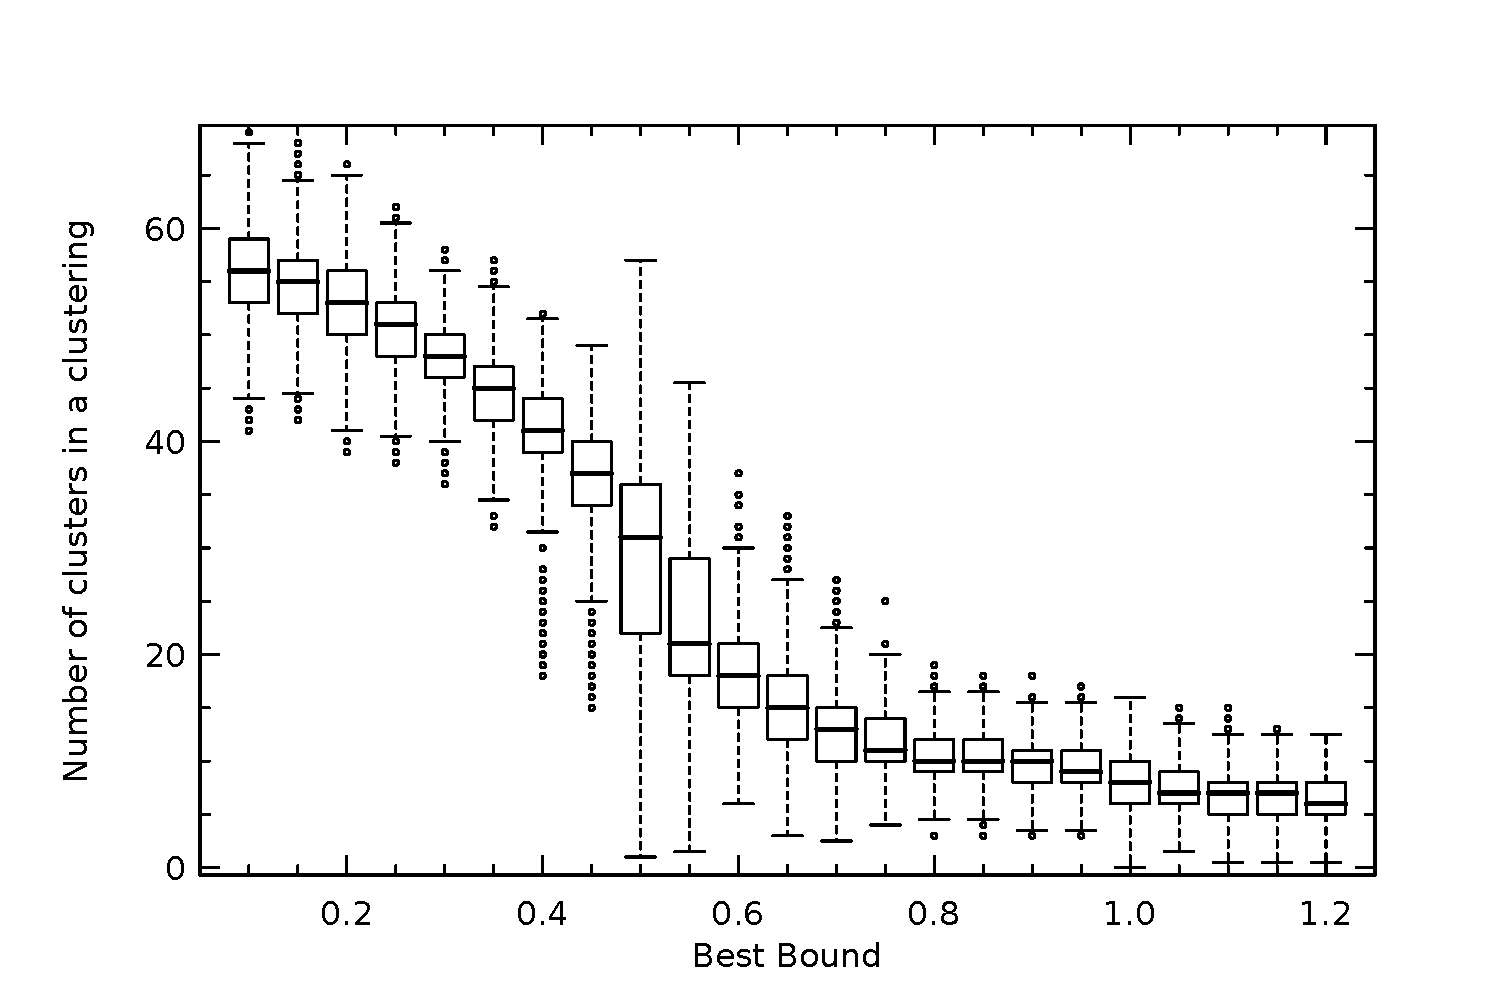
\includegraphics[width=5.5in]{img/mdl-clust_best-bound-cls_1.pdf}
\caption{Size of clusterings (number of clusters in the clustering) produced by LMCLUS algorithm by varying \emph{best\_bound} parameter value.}
\label{fig:best-bound-cls}
\end{figure}



Figure~\ref{fig:best-bound-cls} shows a large variation for clustering sizes
for \emph{best\_bound} in range [0.4,0.7]. This range behaves as a transition
zone between clusterings with a small number of clusters, corresponding to
the large \emph{best\_bound} value, and a large number of clusters,
corresponding to the small \emph{best\_bound} value. We can speculate that for
current dataset algorithm is not able to pick mid range clusters, resulting
in arbitrary partitioning of some large clusters.

\begin{figure}[H]
\center
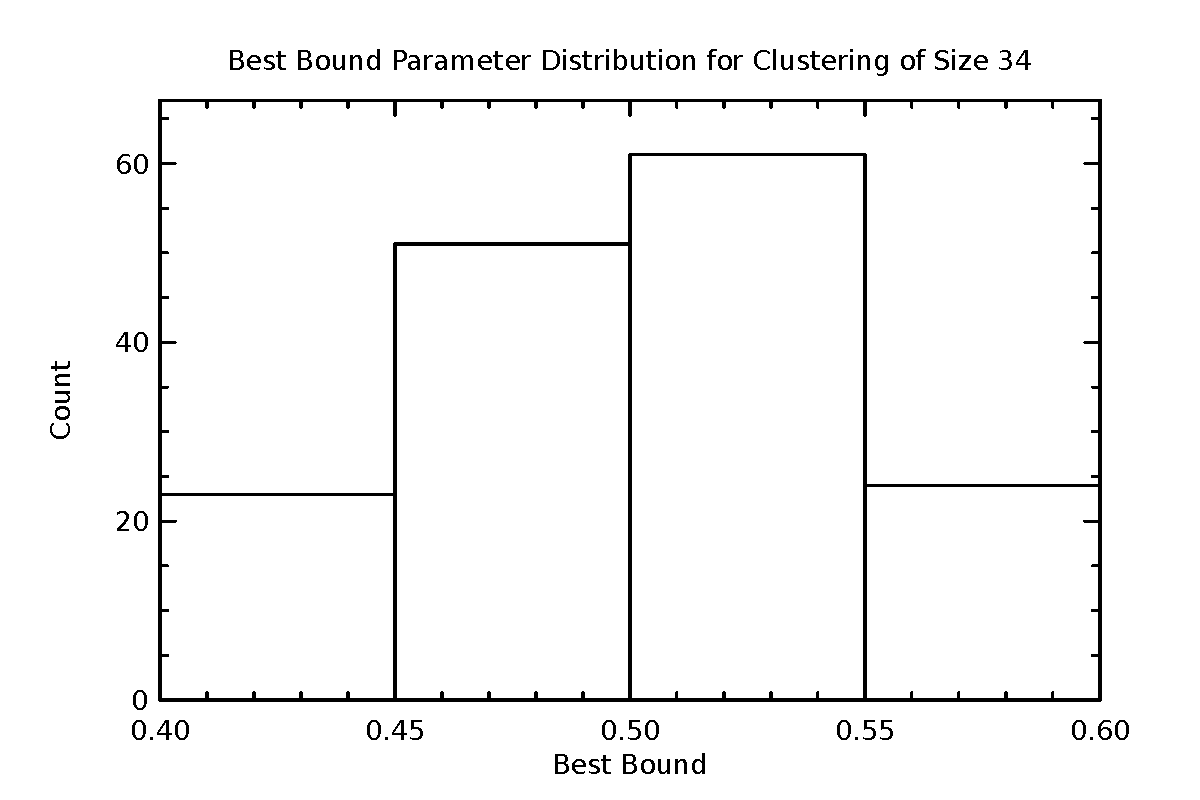
\includegraphics[width=4.5in]{img/mdl-clust_best-bound-cl-34_1.pdf}
\caption{The \emph{best\_bound} parameter value distribution of clustering of size 34.}
\label{fig:best-bound-cl-34}
\end{figure}



Figure~\ref{fig:best-bound-cl-34} shows a distribution of the \emph{best\_bound}
parameter for the clustering size equal to 34, which correspond to the number of
climate zones in K{\"o}ppen-Geiger classification. We can observe that
\emph{best\_bound} parameter is distributed within a "transitional" range where
the clustering algorithm produces clusterings with wide variation of sizes for
given parameters, see Figure~\ref{fig:best-bound-cls}.


Next, we analyze dimensionality of clusters from the sampled clusterings.
Results showed that majority of the clusters in various sized clusterings are
1-dimensional. Usually, the last cluster has dimension zero which is by design -
this cluster is a collection of all outliers that algorithm wasn't able to
associate with any known cluster.
Moreover, a cluster, before last one in a clustering of any size,
has higher dimension then one. This behavior can be attributed to constrained
minimal cluster size, forcing algorithm to generate high-dimensional clusters
with that would pass minimal cluster size threshold, see discussion in
the beginning of Section~\ref{ssc:mdl-clust}.

\begin{figure}[H]
\center
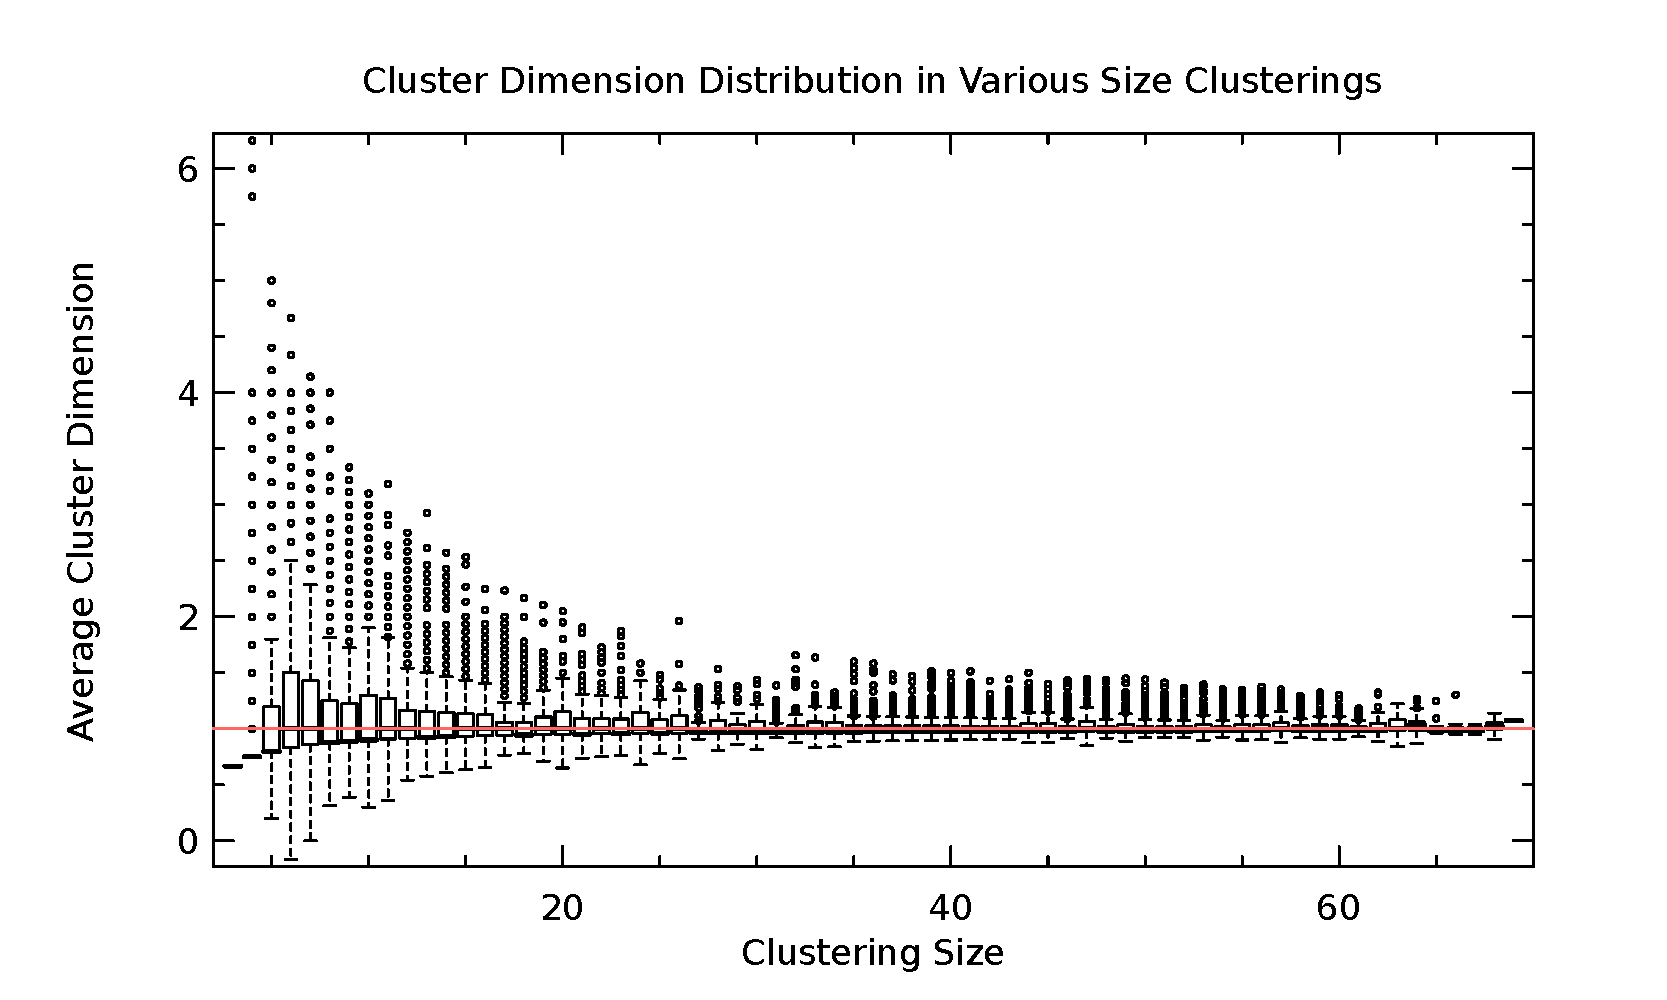
\includegraphics[width=6.0in]{img/mdl-clust_mdl-clust-cdim_1.pdf}
\caption{The \emph{best\_bound} parameter value distribution of clustering of size 34.}
\label{fig:mdl-clust-cdim}
\end{figure}



Figure~\ref{fig:mdl-clust-cdim} shows a cluster dimension distribution for
clusterings of different size. The average dimension of clusters approaches 1
(red line) as number of clusters grows in a clustering. However, there is
a large variability in a cluster dimensionality for small-sized clusterings,
which gradually decreases as the clustering size increases.


In order investigate further occurrence of this pattern, we will look at
the cluster size in generated clusterings. We grouped clusters from
the clusterings of the same size and pooled together corresponded cluster sizes.

\begin{figure}[H]
\center
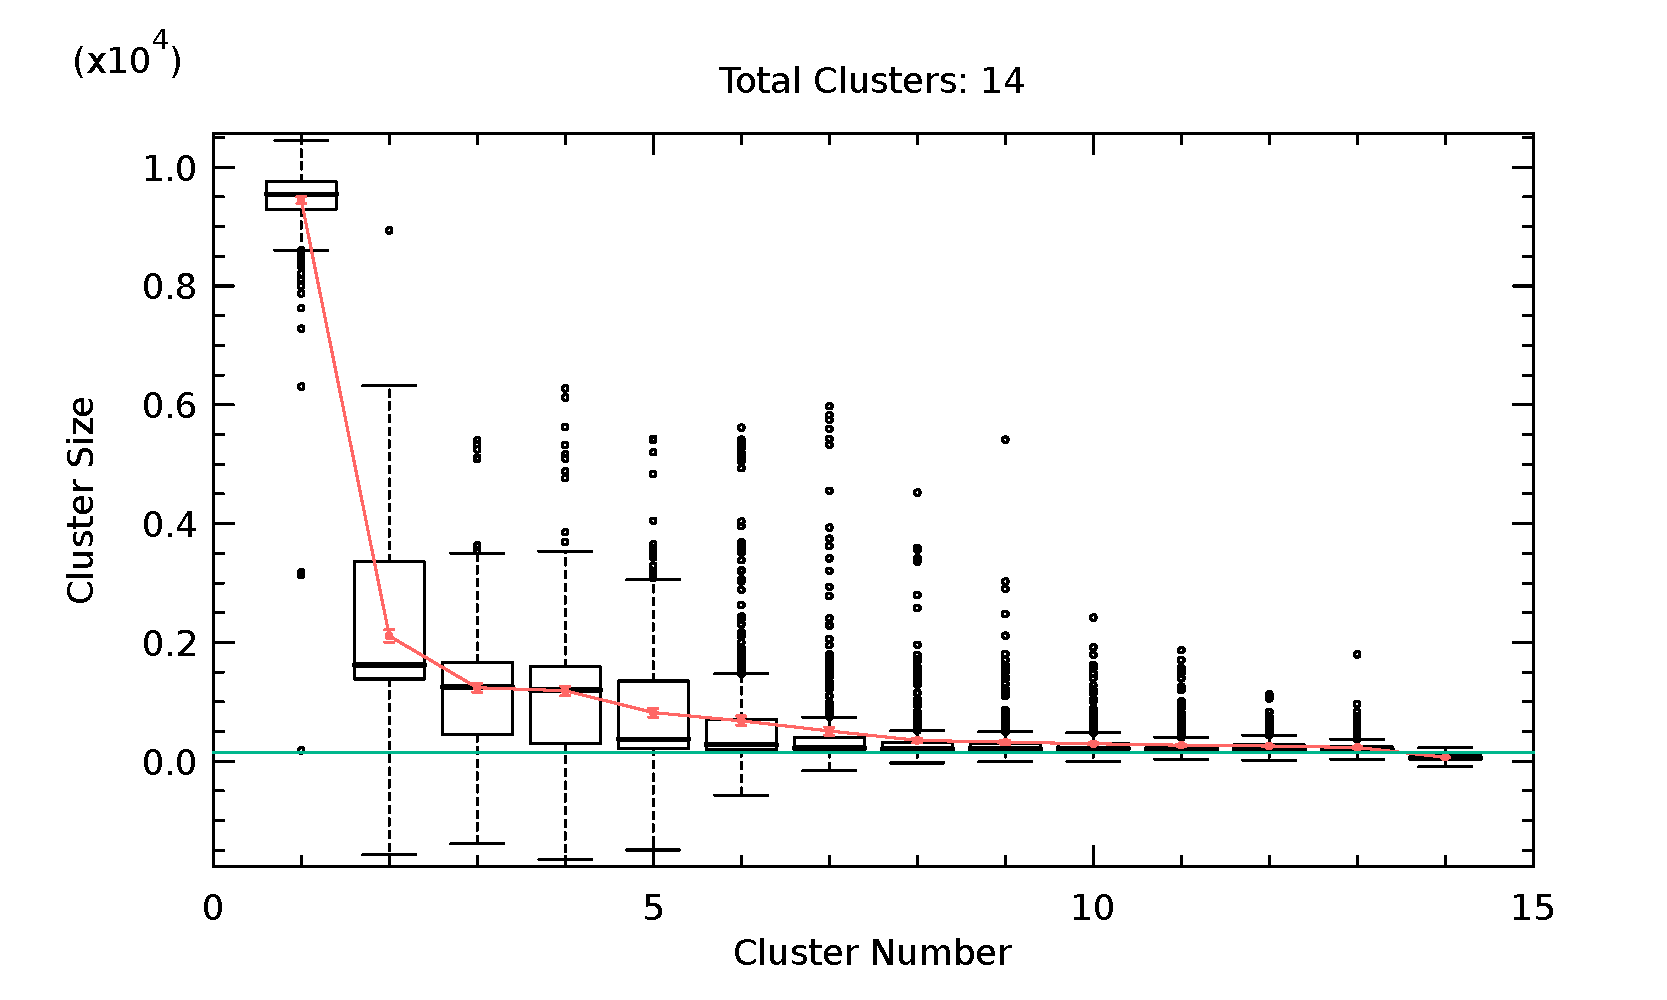
\includegraphics[width=6.0in]{img/mdl-clust_clust-size-14_1.pdf}
\caption{Cluster size distribution for the clustering of size 14.}
\label{fig:clust-size-14}
\end{figure}



Figure~\ref{fig:clust-size-14} shows distribution of the cluster sizes for
clusterings with 14 clusters. The red line on a plot is a bootstrapped mean
cluster size with the corresponding 95\% confidence interval, and the blue line
is a minimal cluster size specified by the LMCLUS parameter,
\emph{min\_cluster\_size}, which is set to 150.

As the number of clusters in the clustering grows, the cluster size  approaches
to the minimal cluster size threshold. Moreover, the cluster size gradually
decreases, for from large clusters, generated at the beginning of
the clustering procedure, to the clusters with the size near the threshold limit
for clusters produced near the end of clustering procedure. This behavior is
observed for all sizes of clusterings, especially with few clusters.


\subsubsection{Clustering MDL Calculations}
\label{sssc:clust-mdl}

In our calculations of MDL values for clusterings, we used following parameters:
an encoding model constant, $P_m$, set to 32, an encoding data constant,
$P_d$, set to 16, and the user-defined quantization error upper boundary,
$\varepsilon$, set to 0.001.




In two-part MDL calculation for linear manifold clusters, first part, a cluster
model description is computed by \eqref{eq:mdl-lmc-model},
$L(\mathcal{M}) = P_m N (N+1)/2$.
However, when cluster is not of a linear manifold form, we calculate its
description as if it's a spherical cluster. Thus, we only need to encode center
of the spherical cluster in a model description, $L(\mathcal{M}) = P_m N$.

\begin{figure}[H]
\center
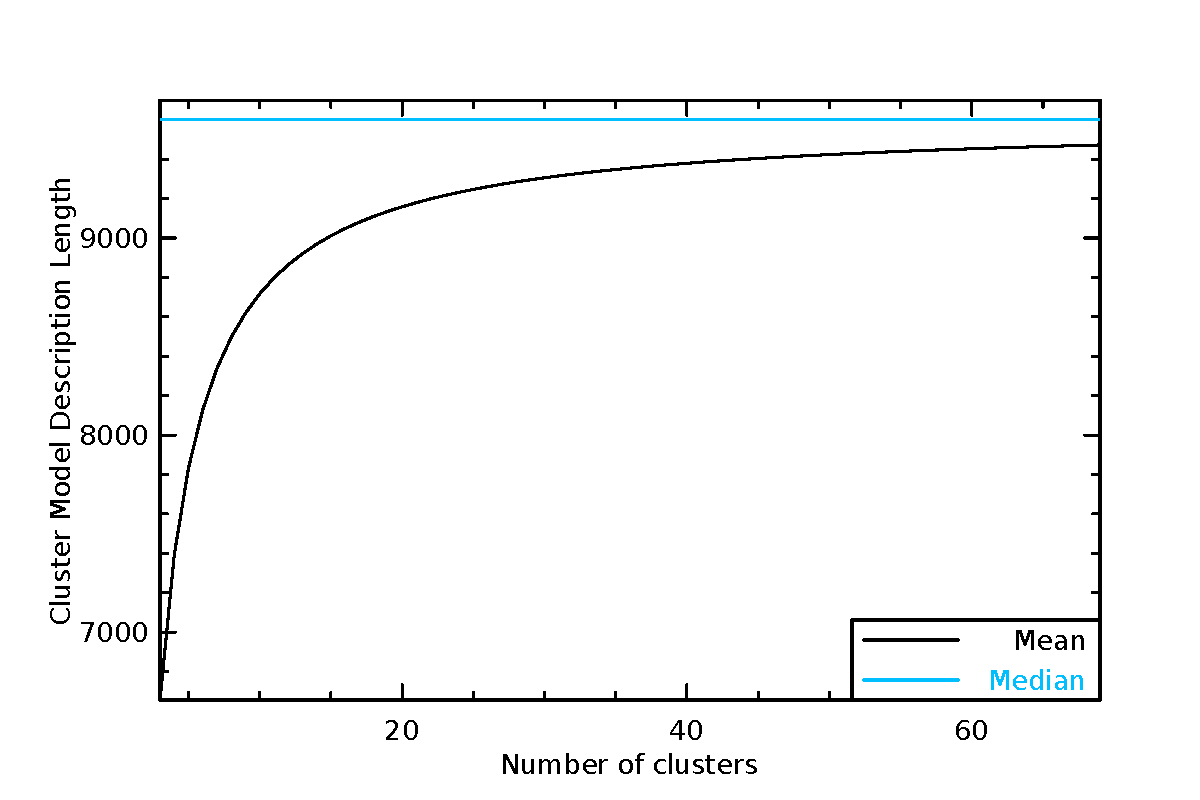
\includegraphics[width=5.0in]{img/mdl-clust_model-dl-stats_1.pdf}
\caption{Cluster model description length mean amd median values.}
\label{fig:model-dl-stats}
\end{figure}



Figure~\ref{fig:model-dl-stats} shows mean and median model description length
values for sampled clusterings grouped by their size. The model MDL for
1-dimensional LM cluster is 32 x 24 x 25/2 = 9600. As expected, a median MDL for
a clusters in sampled clusterings is 9600 bits, which corresponds to MDL value
of the dominant cluster in all generated clustering samples. A mean cluster
model MDL value is expected to approach median value. As almost every clustering
contains a 0-dimension cluster of outliers, the more clusters in the clustering,
the closer average model MDL value to the model MDL of 1-dimensional LM cluster.

In context of the MDL calculation for a clustering, the total model MDL of
a clustering $\mathcal{K}$, composed of $k$ clusters, is calculated as

$$L(\mathcal{K}) = \sum_k L(\mathcal{M}_k)$$

Thus, we should expect linear grows of the clustering model MDL value with
a number of clusters, because every cluster has only one 0-dimensional "noise"
cluster and the rest of the clusters are described by constant number of bits,
see Figure~\ref{fig:clustering-model-dl}.

\begin{figure}[H]
\center
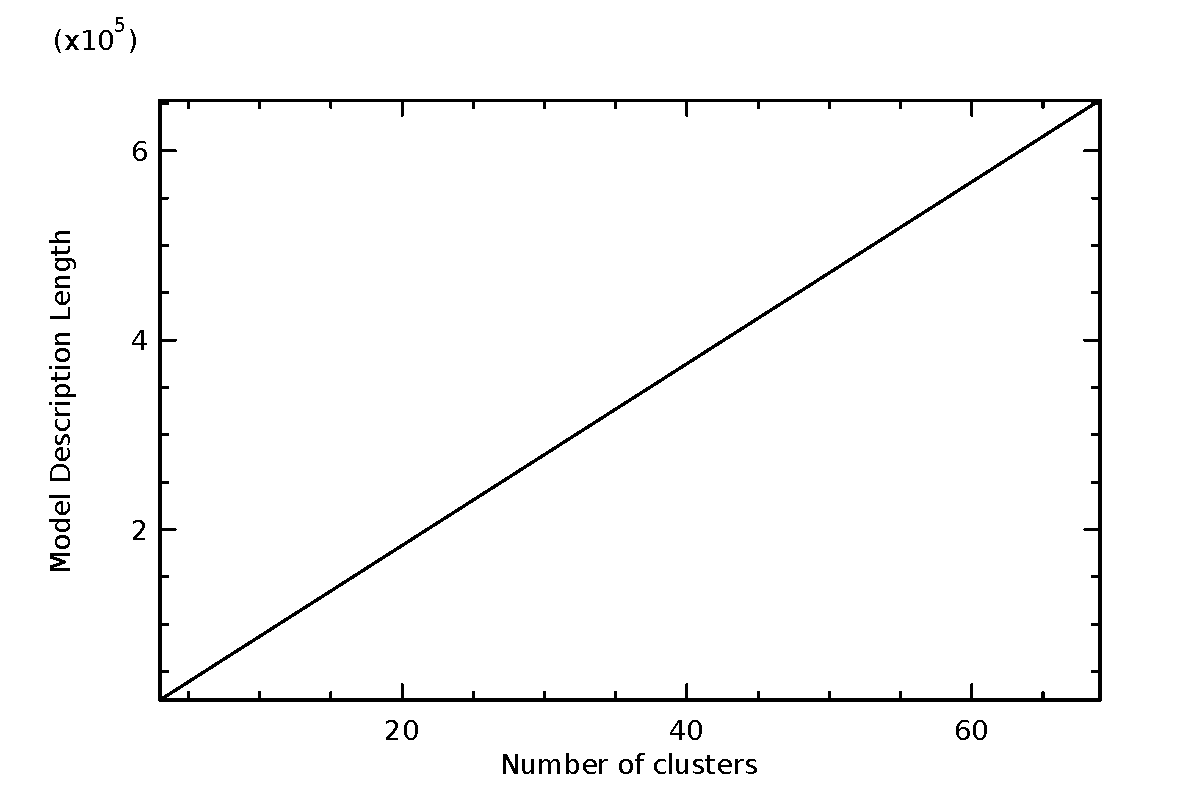
\includegraphics[width=4.0in]{img/mdl-clust_clustering-model-dl_1.pdf}
\caption{Clustering Model Description Length.}
\label{fig:clustering-model-dl}
\end{figure}



In context of the MDL calculation for a clustering, a total data MDL value of
a clustering $\mathcal{K}$, composed of $k$ clusters, is calculated as

\begin{equation}
L(D \;|\;\mathcal{K}) = \sum_k L(\mathcal{C_k} \;|\;\mathcal{M_k}) = \sum_k P_d M_k J_k + \sum_k J_k S_{k, M_k}(\varepsilon)
\end{equation}

where $L(\mathcal{C} \;|\;\mathcal{M})$ is a description length of the cluster
$\mathcal{C}$ encoded given the model $\mathcal{M}$, see \eqref{eq:mdl-lmc-data}.




If size of the dataset $D$ is $d = |D| = \sum_k J_k$, then first term,
$\sum_k P_d M_k J_k$ can be approximated with $(P_d d) E[M]$,
where $E[M]$ is an expected value of the cluster dimensionality in a particular
clustering, and $d = \sum_k J_k$ is a size of the dataset.
Second term, $\sum_k J_k S_{k, M_k}$ can be views as expected values of
the entropy of the OSC points distribution $(d)E[S]$, so

$$L(D \;|\;\mathcal{K}) = (P_d d) E[M] + (d) E[S]$$

We also would like to compare data MDL of the clustering when all components are
just encoded with entropy, as in case of MDL calculation for a zero-dimensional
cluster.

$$L_z(D \;|\;\mathcal{K}) = (d)E[S]$$

Figure~\ref{fig:clustering-data-dl} shows a distribution of the clustering data
MDL values, $L(D \;|\;\mathcal{K})$, as a box plot, and bootstrapped mean value
of $L(D \;|\;\mathcal{K})$, as well as bootstrapped mean value of a clustering
entropy from all components of the cluster points, $L_z(D \;|\;\mathcal{K})$.

\begin{figure}[H]
\center
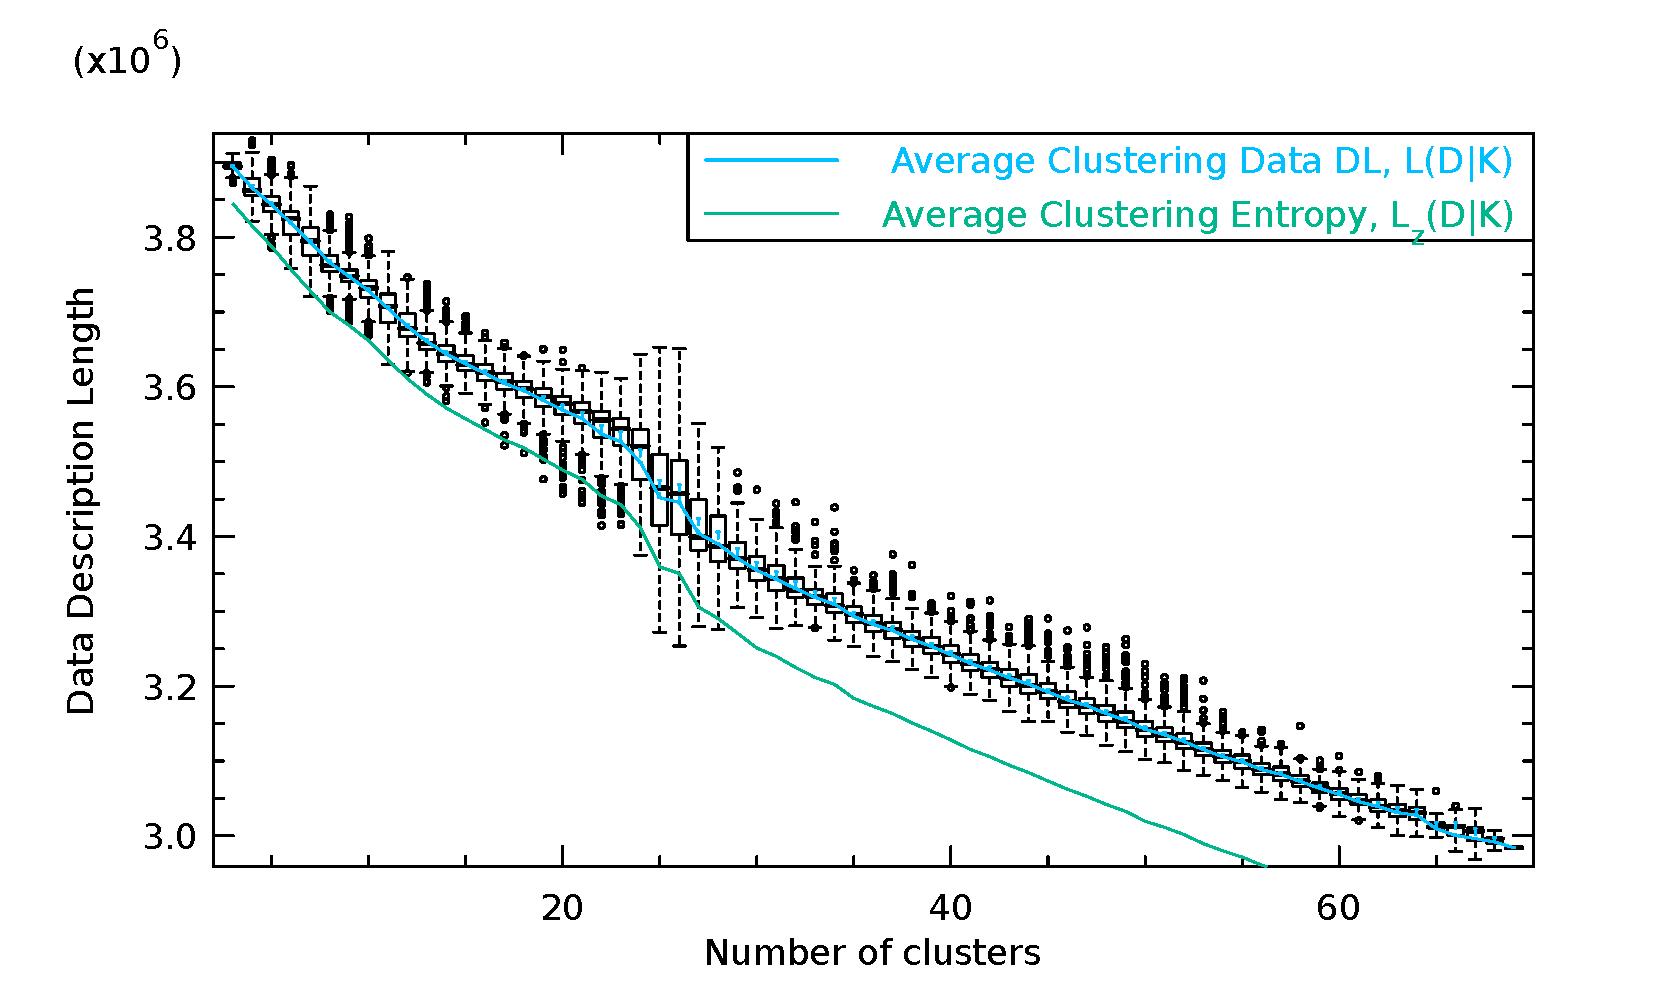
\includegraphics[width=5.0in]{img/mdl-clust_clustering-data-dl_1.pdf}
\caption{Clustering Data Description Length.}
\label{fig:clustering-data-dl}
\end{figure}



Displayed pattern shows expected linear downward trend: when the number of
clusters increases in the clustering, the clustering MDL value tend to decrease.
This happens because clusters become more compact and encoding is better for
such clusters yielding smaller MDL value. There is only one discrepancy in
the clustering size interval of [20,30]. It can be attributed to large cluster
dimensionality variation for clustering with particular number of clusters.

Now, we can calculate clustering MDL for the dataset $D$ by combining two parts:
$L(\mathcal{K})$ and $L(D \;|\;\mathcal{K})$.
We predicted that with that two-parted linear manifold MDL, we would have
large MDL value when the clustering has few clusters, which is driven by large
\emph{data}-part of joint MDL value for small-sized clusterings,
as well as large MDL value when the clustering has many clusters, which is
driven by large \emph{model}-part MDL value for large-sized clusterings.
Between these MDL value extrema, we should have clustering with minimal MDL
value characterized by balancing model and data MDL parts.

\begin{figure}[H]
\center
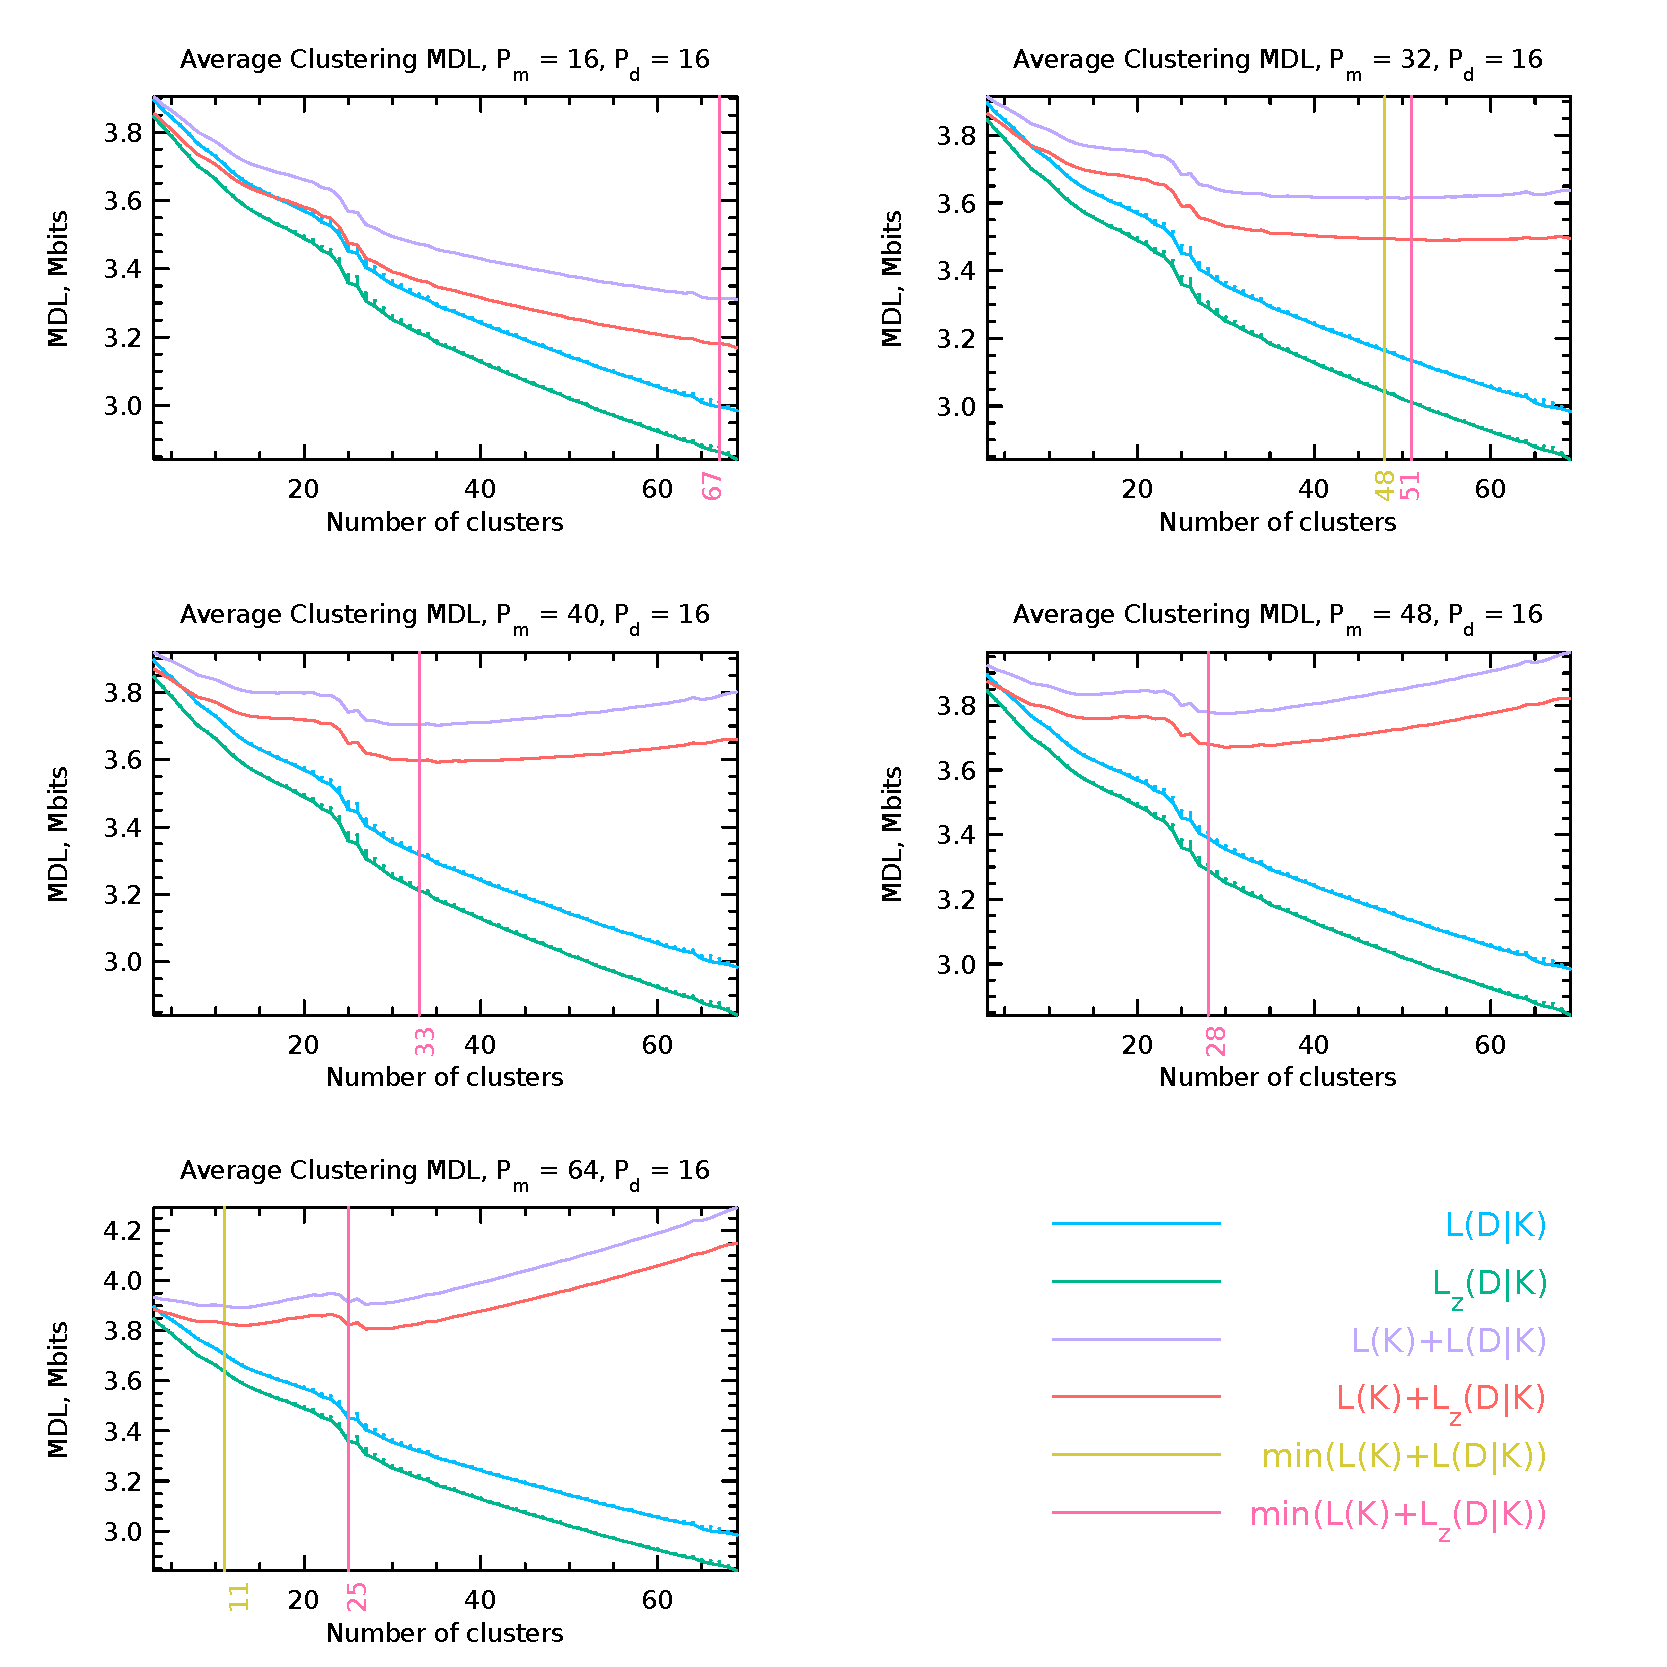
\includegraphics[width=5.0in]{img/mdl-clust_clustering-mdl_1.pdf}
\caption{Avarage Clustering MDL for different encoding constant values.}
\label{fig:clustering-mdl}
\end{figure}



Figure~\ref{fig:clustering-mdl} shows plots of average two-part MDL values and
data MDL values (as well as MDL value based on cluster entropy) for clusterings
of different size. Vertical lines on plots identify clustering sizes which are
corresponded to the minimal MDL value under particular parameters.
We generated these plots for various $P_m$ constants, in order to see how these
constant would affect total MDL value, as it is primary parameter for the model
MDL calculation.

We found that with default parameters $P_m = 32$ and $P_d = 16$, the clustering
MDL value levels on after clustering size 30, reaching minimum value for
the clustering with 51 cluster and then gradually increases. With $P_m < 32$,
the clustering MDL value continues to decrease and we are not able to determine
correctly minimal MDL as we have a little or no data for clustering size beyond
67 clusters. With $P_m > 32$, we could clearly identify the minimal MDL value
and see its increase as clustering size grows.

Notably, $P_m = 40$ lands minimum clustering MDL for clusterings with
33 clusters which is very close to the expected value of 34 climate classes from
the K{\"o}ppen-Geiger (KG) climate classification.

\begin{figure}[H]
\center
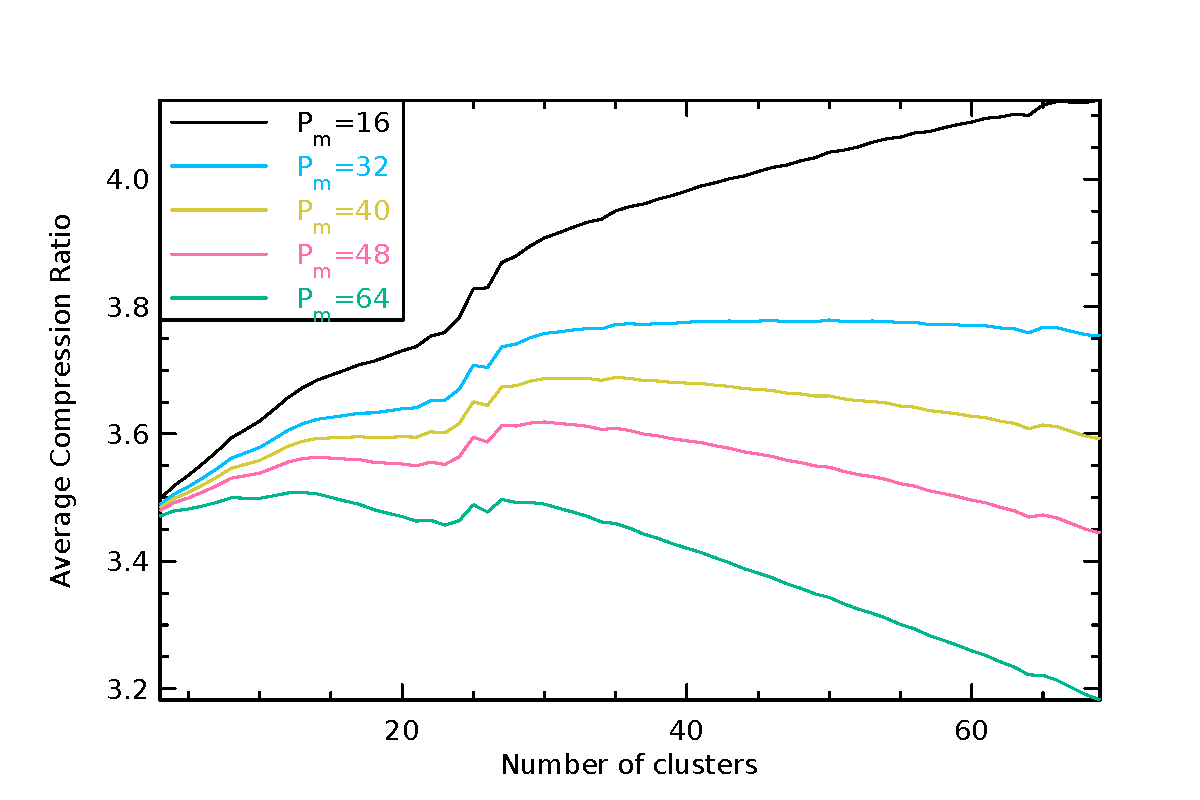
\includegraphics[width=5.0in]{img/mdl-clust_clustering-mdl-cr_1.pdf}
\caption{Average clustering MDL compression ratio.}
\label{fig:clustering-mdl-cr}
\end{figure}



Figure~\ref{fig:clustering-mdl-cr} shows average compression ration calulated
for various model encoding constants.
Using average clustering MDL, we can evaluate some of the parameters of
the MDL heuristics for LMCLUS algorithm such as the encoding constants,
$P_d$ and $P_m$, and the compression ratio. Compression ratio defines the ratio
between an uncompressed (raw) encoding of the dataset with constant precision,
$P_r$ and a clustering MDL  which is an encoding of the dataset using
a particular clustering partition. It's calculated as follows
$$CR = \frac{P_rNd}{MDL}$$
where $P_r = 32$ is a precision encoding constant for raw data, $N$ is dataset dimension, and $d$ is a size of the dataset.

\fi
\section{Conclusion}
\label{sc:conclusion}

We described a novel regularization technique for the linear manifold clustering
based on the idea that a linear manifold shaped cluster allows efficient compression
of the cluster data to the degree allowed by the specified error threshold.
This intuitive criterion was formalized as the minimization problem of
the description length of a prospective cluster and incorporated into
the stochastic search of the clustering algorithm.

In the empirical part of the work we studied the behavior of the proposed MDL
encoding, and the effect of the quantization error on it. We confirmed that
the described method produced reasonable results for simulated datasets, as
well as on the climate data clustering task. We believe that this regularization
technique allows creation of clusters that are more informative and
comprehensive.

A comprehensive scoring of the clusters with MDL values provides not only a
criteria for cluster goodness-of-fit evaluation, but as well can be viewed as
a qualitative measure which is used to explore stability of the clustering
algorithm \cite{VonLuxburg:2005VB}, or to improve clustering performance by
introducing a scoring function for a guided stochastic search, which is left to
be explored in our future research.

% Bibliography
\bibliographystyle{plain}
\bibliography{inexact_mdl_lmc}

\newpage
% Appendix
\begin{appendices}
\renewcommand{\thesubsection}{\Alph{subsection}}
\subsection{Understanding the Results of Linear Manifold Clustering}
\label{ssec:lmclus-results}

%TODO: wrong \lambda_n^2 < \theta^2
Let the measurement space be $R^N$ and the data set, consisting of
a list of observations from $R^N$, be $D$. A linear manifold cluster
$C$ of dimension $K$ is defined by
\begin{eqnarray*}
C=\{x\in D\ &|&\ \mbox{ for some }\lambda_1,\ldots,\lambda_N,\\
 && x=\mu+\sum_{n=1}^N \lambda_n\alpha_n \mbox{ where }\\
&&      \sum_{k=K+1}^N \lambda_n^2 < \theta^2\}
\end{eqnarray*}

$\mu$ is the center of the cluster so it is the vector that translates
the origin to the center of the manifold. It is computed as the mean of the
data vectors that are in the cluster.

\begin{eqnarray*}
\mu&=&\frac{1}{|C|}\sum_{x\in C} x
\end{eqnarray*}


$\alpha_1,\ldots,\alpha_N$ are an orthonormal basis for $R^N$ and
$\alpha_1,\ldots,\alpha_K$ constitute the basis for the $K$-dimensional
manifold.

For any $x\in C$, the corresponding $\lambda_1,\ldots,\lambda_N$ are given
by
\begin{eqnarray*}
\lambda_n&=&\alpha_n^\prime(x-\mu)
\end{eqnarray*}

The linear manifold bounding box $B$ is given by

\begin{eqnarray*}
B=\{x\in R^N\ &|&\ \mbox{ for some } \lambda_1,\ldots,\lambda_K,
 x=\mu+\sum_{k=1}^K \lambda_k\alpha_k \\
 \mbox{ where }\lambda_{kmin}\le&\lambda_k& \le \lambda_{kmax} \\
\lambda_{kmin}&=&\min_{x\in C} \alpha_k^\prime(x-\mu), k=1,\ldots,K\\
\lambda_{kmax}&=&\max_{x\in C} \alpha_k^\prime(x-\mu), k=1,\ldots,K\}\\
\end{eqnarray*}

The constants $\lambda_{kmin}$ and $\lambda_{kmax}$ determine the extent
of the boundary of the bounding box in dimension $k$ whose basis vector is $\alpha_k$.

To show the distribution of the points in the cluster, we show the histogram
of the data orthogonally projected onto each basis vector of the cluster.
Let $D_k$ be list of the projections on the $k^{th}$ axis. Then
\begin{eqnarray*}
D_k&=&< a\in [\lambda_{kmin},\lambda_{kmax}] \ | \ \mbox{ for some } x\in C,\ a=\alpha_k^\prime(x-\mu)>
\end{eqnarray*}

If the histogram of the $k^{th}$ axis has $M$ intervals, $[\eta_m,\eta_{m+1}], m=1\ldots,M$
then
\begin{eqnarray*}
\eta_m&=&\lambda_{kmin}+ \frac{(m-1)}{M}(\lambda_{kmax}-\lambda_{kmin})
\end{eqnarray*}
The probability $p_m$ that a data point of the cluster is in interval $[\eta_m,\eta_{m+1}]$
is given by
\begin{eqnarray*}
p_m&=&\frac{1}{\#D_k} \# < x\in C\ | \ \eta_m \le \alpha_k^\prime(x-\mu) \le \eta_{m+1}>
\end{eqnarray*}

The $M$ heights of the histogram $H_k$ of the $k^{th}$ axis is then given by
$p_1,\ldots,p_M$.
These $K$ histograms then give a first order picture of how the data is distributed
on the manifold in the reference frame of the manifold.

Of course the observed data points are not, in general, on the cluster manifold.
Rather, they are close to the manifold. The distance $\rho$ of an observed data point
$x$ from the manifold is given by

\begin{eqnarray*}
\rho(x)&=&\sqrt{\sum_{k=K+1}^N [\alpha_k^\prime (x-\mu)]^2}\\
&=& \sqrt{(x-\mu)^\prime(x-\mu)-\sum_{k=1}^K[\alpha_k^\prime (x-\mu)]^2}
\end{eqnarray*}

If there are $M$ intervals to the histogram and the $m^{th}$ interval
is $[\delta_m,\delta_{m+1}]$, then

\begin{eqnarray*}
\delta_m=\rho_{min}+\frac{m-1}{M}(\rho_{max}-\rho_{min})
\end{eqnarray*}
where
\begin{eqnarray*}
\rho_{min}&=&\min_{x\in C}\rho(x)\\
\rho_{max}&=&\theta
\end{eqnarray*}

The heights $q_1,\ldots,q_M$ of the histogram $H$ are given by

\begin{eqnarray*}
q_m&=&\frac{1}{\#C}<x\in C\ | \ \delta_m \le \rho(x) \le \delta_{m+1},\ m=1,\ldots,M>
\end{eqnarray*}
This histogram shows the spread of the data off the manifold.

To complete the information of the cluster, the vectors
\begin{itemize}
\item $\mu$
\item $\alpha_1,\ldots,\alpha_K$
\end{itemize}
must be given.

For those people who would like to understand the linear manifold cluster
in terms of a set of constraint equations, define

\begin{eqnarray*}
B&=&\left(\begin{array}{c}
               \alpha_{K+1}^\prime\\
               \alpha_{K+2}^\prime\\
               \vdots\\
               \alpha_{N}^\prime
               \end{array}\right)
\end{eqnarray*}

Then the constraint equation for the manifold of the cluster is given by

\begin{eqnarray*}
B(x-\mu)&=&0
\end{eqnarray*}
 % Understanding the Results of LMCLUS
\newpage
\subsection{LMCLUS Algorithm Parameters} \label{ssec:lmclus-params}
\mbox{}

\begin{longtable}[H]{@{\extracolsep{\fill}}lp{4in}p{.7in}@{}}
\caption{List of LMCLUS algorithm parameters} \label{tab:lmclus-params} \\

\toprule\addlinespace
\textbf{Parameter} & \textbf{Description} & \textbf{Default value} \\
\midrule\addlinespace
\endfirsthead

\multicolumn{3}{c}%
{{\bfseries \tablename\ \thetable{} (continued)}} \\
\toprule\addlinespace
\textbf{Parameter} & \textbf{Description} & \textbf{Default value} \\
\midrule
\endhead

\addlinespace
\midrule
\multicolumn{3}{r}{\textbf{Continued on next page}} \\
\endfoot

\hline \hline
\endlastfoot

% Table of parameters

min\_dim & Minimum dimensionality of manifolds & $\leq N-1$ \\ \addlinespace

max\_dim & Maximum dimensionality of manifolds & $\leq N-1$ \\ \addlinespace

number\_of\_clusters & Estimate and specify nominal number of resulting clusters & 100 \\ \addlinespace

min\_cluster\_size & Minimum cluster size (or noise size) in order to prevent generation of small clusters & 50 \\ \addlinespace

random\_seed & Random generator seed value. & \\ \addlinespace

sampling\_heuristic & Choose sampling heuristics for the linear manifold
basis selection. There are three modes of the sampling:
\begin{enumerate}
\item algorithm will use a probabilistic heuristic which will sample a quantity
exponential in `maximum cluster dimension' and `maximum number of
clusters' parameters;
\item will sample fixed number of points based on `sampling\_factor' parameter;
\item the lesser of the previous two.
\end{enumerate}
& 3 \\ \addlinespace

sampling\_factor & Sampling factor used in the sampling heuristics to constrain a number of samples to fixed value. It is equal to an inspected-at-the-moment dataset size multiplied to a this parameter value. & 0.01 \\ \addlinespace

hist\_bin\_size & Fixed number of bins for the distance histogram. If this parameter is set to zero then proportional selection of a histogram bin number is used & 0 \\ \addlinespace

max\_bin\_portion & Maximum histogram bin size as a portion. If the number of bins for the distance histogram is not specified, it is calculated proportionally to the dataset size. & 0.1 \\ \addlinespace

histogram\_sampling & Turns on a sampling for a distance histogram. Instead of computing the distance histogram from whole dataset, algorithm draws smaller sample for the histogram construction. & false \\ \addlinespace

error\_bound & Sampling error bound determines a minimal number of samples required to correctly identify a linear manifold cluster. & 0.0001 \\ \addlinespace

best\_bound & Separation best bound value is used for evaluating a goodness of separation characterized by a discriminability and a depth between modes of a distance histogram. & 1.0 \\ \addlinespace

mdl & Enables the minimum description length (MDL) heuristic for a complexity validation of a generated cluster & false \\ \addlinespace

mdl\_model\_precision & MDL heuristic requires to specify a model precision encoding constant. & 32 \\ \addlinespace

mdl\_data\_precision & MDL heuristic requires to specify a data precision encoding constant. & 16 \\ \addlinespace

mdl\_quant\_error & Quantizing error of a bin size calculation for a histogram which used in determining entropy value of the empirical distance distribution. & 0.001 \\ \addlinespace

mdl\_compres\_ratio & Quantizing error of a bin size calculation for a histogram which used in determining entropy value of the empirical distance distribution. & 1.05 \\ \addlinespace

basis\_alignment & Turn of/off an alignment of a manifold cluster basis. If it's on, a manifold basis of the generated cluster is aligned along the direction of the maximum variance (by performing PCA). & false \\ \addlinespace

dim\_adjustment & Turn of/off a linear manifold cluster dimensionality detection by looking for portion of a variance associated with principal components. & false \\ \addlinespace

dim\_adjustment\_ratio & Ratio of manifold principal subspace variance. & 0.99 \\ \addlinespace

\bottomrule
\end{longtable}
  % LMCLUS parameters
% \if\CommandLineArg1
% \newpage
% \input{cluster-plots}  % Plot cluster points scattergrams
% \fi
\end{appendices}

\end{document}
